\input{setup/preamble.tex}% package inclusion and set up of the document

%this package must be included
%in a file which is open during any session
%otherwise \autoref will not autocomplete
\usepackage{hyperref}

%%%%%%%%%%%%%%%%%%%%%%%%%%%%%%%%%%%%%%%%%%%%%%%%%%%%%
%             UNITS, EQUATIONS AND TEXT             %
%%%%%%%%%%%%%%%%%%%%%%%%%%%%%%%%%%%%%%%%%%%%%%%%%%%%%

%%Macro for 'where'enviroment has been improved by Andrea :-)

%Units:
\newcommand{\unit}[1]{&& \left[\si{#1}\right]} %\newcommand{\unit}[1]{[\si{#1}]}             <<| Use these if you want equations to be
\newcommand{\unitWh}[1]{[\si{#1}]}             %\newcommand{\eq}[2]{&&\si{#1} &= \si{#2}&&}  <<| centered.. .. will appear scrambled
\newcommand{\numUnit}[1]{\ \si{#1}&}           %                                               | from one equation to the next though..
%Equation:                                     %                                               | and does not work with long equations.. :/
\newcommand{\eq}[2]{\si{#1} &= \si{#2}}
\newcommand{\arw}{&& &\Updownarrow&&}
\newcommand{\eqOne}[2]{\si{#1} &= \si{#2} &\nonumber\\}
\newcommand{\eqTwo}[1]{&\ \ \ \ \si{#1}&}
\newcommand{\eqThree}[1]{&\ \ \ \ \si{#1}&}
%Text:
\newcommand{\tx}[1]{\text{#1}}
%Vectors
\renewcommand{\vec}[1]{\boldsymbol{\mathbf{#1}}}

%Vertical line in equations ie. |_x=y (whereTwo stacks two equalities at the line)
\newcommand{\whereOne}[1]{ \left.\rule{0cm}{.7cm}\right\vert\rule{0cm}{.7cm}_{\substack{\rule{0cm}{.28cm}\\ #1 }} }
\newcommand{\whereTwo}[2]{ \left.\rule{0cm}{.7cm}\right\vert\rule{0cm}{.7cm}_{\substack{#1 \rule{0cm}{.2cm}\\\vspace{-.1cm}\\ #2}} }
\newcommand{\whereThree}[3]{ \left.\rule{0cm}{1cm}\right\vert\rule{0cm}{1cm}_{\substack{\\\vspace{-.1cm}\\ #1 \rule{0cm}{.1cm}\\\vspace{-.1cm}\\ #2 \rule{0cm}{.1cm}\\\vspace{-.1cm}\\ #3}} }





%%%%%%%%%%%%%%%%%%%%%%%%%%%%%%%%%%%%%%%%%%%%%%%%%%%%%
%              SETTING UP NOTE BOXES                %
%%%%%%%%%%%%%%%%%%%%%%%%%%%%%%%%%%%%%%%%%%%%%%%%%%%%%
%\specialcomment{note}{\[}{\]}
%%{\begin{tcolorbox}
%%                      [grow to right by  = 1.5 cm
%%                      ]}{\vspace{-.3 cm}\end{tcolorbox}}
%
%\newcommand{\toggleNotes}[1]
%{
%  \ifthenelse{\equal{#1}{off}}{\excludecomment{note}}{}
%}

%%%%%%%%%%%%%%%%%%%%%%%%%%%%%%%%%%%%%%%%%%%%%%%%%%%%%
%                 TIKZ SETTINGS                     %
%%%%%%%%%%%%%%%%%%%%%%%%%%%%%%%%%%%%%%%%%%%%%%%%%%%%%
%\usetikzlibrary{arrows.meta}
\tikzset{
  block/.style    = {draw, thick, rectangle,
                     minimum height = 2.1em,
                     minimum width = 1.7em},
  sum/.style      = {draw, circle, inner sep=1.5pt},
}

%%%%%%%%%%%%%%%%%%%%%%%%%%%%%%%%%%%%%%%%%%%%%%%%%%%%%
%                  REFERENCES                       %
%%%%%%%%%%%%%%%%%%%%%%%%%%%%%%%%%%%%%%%%%%%%%%%%%%%%%

%Chapter
\newcommand{\Chapref}[1]{\emph{Chapter \ref{#1}}}
\newcommand{\chapref}[1]{\emph{chapter \ref{#1}}}
%Section
\newcommand{\Secref}[1]{\emph{Section \ref{#1}}}
\newcommand{\secref}[1]{\emph{section \ref{#1}}}
%subSection
\newcommand{\Subsecref}[1]{\emph{Subsection \ref{#1}}}
\newcommand{\subsecref}[1]{\emph{subsection \ref{#1}}}
%Appendix
\newcommand{\Appref}[1]{\emph{Appendix \ref{#1}}}
\newcommand{\appref}[1]{\emph{appendix \ref{#1}}}
%Listings
\newcommand{\Coderef}[1]{\emph{Listings: \ref{#1}}}
\newcommand{\coderef}[1]{\emph{listings: \ref{#1}}}
%Figure:
\newcommand{\Figref}[1]{\emph{Figure \ref{#1}}}
\newcommand{\figref}[1]{\emph{figure \ref{#1}}}
%Table:
\newcommand{\Tableref}[1]{\emph{Table \ref{#1}}}
\newcommand{\tableref}[1]{\emph{table \ref{#1}}}

%Expressions:
\newcommand{\Expr}[1]{\emph{Expression (\ref{#1})}}
\newcommand{\expr}[1]{\emph{expression (\ref{#1})}}

%Equations:
%1 equation:
\newcommand{\Eqref}[1]{\emph{Equation (\ref{#1})}}
\renewcommand{\eqref}[1]{\emph{equation (\ref{#1})}}
%2 equations:
\newcommand{\EqrefTwo}[2]{\emph{Equation (\ref{#1})} and \emph{(\ref{#2})}}
\newcommand{\eqrefTwo}[2]{\emph{equation (\ref{#1})} and \emph{(\ref{#2})}}
%3 equations:
\newcommand{\EqrefThree}[3]{\emph{Equation (\ref{#1})}, \emph{(\ref{#2})} and \emph{(\ref{#3})}}
\newcommand{\eqrefThree}[3]{\emph{equation (\ref{#1})}, \emph{(\ref{#2})} and \emph{(\ref{#3})}}
%4 equations:
\newcommand{\EqrefFour}[4]{\emph{Equation (\ref{#1})}, \emph{(\ref{#2})}, \emph{(\ref{#3})} and \emph{(\ref{#4})}}
\newcommand{\eqrefFour}[4]{\emph{equation (\ref{#1})}, \emph{(\ref{#2})}, \emph{(\ref{#3})} and \emph{(\ref{#4})}}
%5 equations:
\newcommand{\EqrefFive}[5]{\emph{Equation (\ref{#1})}, \emph{(\ref{#2})}, \emph{(\ref{#3})}, \emph{(\ref{#4})} and \emph{(\ref{#5})}}
\newcommand{\eqrefFive}[5]{\emph{equation (\ref{#1})}, \emph{(\ref{#2})}, \emph{(\ref{#3})}, \emph{(\ref{#4})} and \emph{(\ref{#5})}}
%6 equations:
\newcommand{\EqrefSix}[6]{\emph{Equation (\ref{#1})}, \emph{(\ref{#2})}, \emph{(\ref{#3})}, \emph{(\ref{#4})}, \emph{(\ref{#5})} and \emph{(\ref{#6})}}
\newcommand{\eqrefSix}[6]{\emph{equation (\ref{#1})}, \emph{(\ref{#2})}, \emph{(\ref{#3})}, \emph{(\ref{#4})}, \emph{(\ref{#5})} and \emph{(\ref{#6})}}
%7 equations:
\newcommand{\EqrefSeven}[7]{\emph{Equation (\ref{#1})}, \emph{(\ref{#2})}, \emph{(\ref{#3})}, \emph{(\ref{#4})}, \emph{(\ref{#5})}, \emph{(\ref{#6})} and \emph{(\ref{#7})}}
\newcommand{\eqrefSeven}[7]{\emph{equation (\ref{#1})}, \emph{(\ref{#2})}, \emph{(\ref{#3})}, \emph{(\ref{#4})}, \emph{(\ref{#5})}, \emph{(\ref{#6})} and \emph{(\ref{#7})}}


\newcommand{\newpar}{\par \vspace{0.4cm}}


%\usepackage{xifthen}
%
%\newenvironment{where}{\indent Where:\\}{}
%\newcommand{\va}[3]
%{
%  \hspace{-18mm}
%  \begin{tabular}{p{35pt} p{345pt} l}
%    { $#1$ } & { #2 } & \ifthenelse{\isempty{ #3 }}  {}  {\si{[#3]}}
%  \end{tabular}
%}















\usetikzlibrary{calc}
\usetikzlibrary{backgrounds}
\newcommand{\showgrid}{%
  \AtBeginShipoutNext{\AtBeginShipoutAddToBoxForeground{%
      \begin{tikzpicture}
        [
          overlay,
          remember picture,
          inner sep=0pt,
          outer sep=0pt,
          minor line/.style={help lines, draw=gray!25, on background layer},
          major line/.style={help lines, draw=gray},
        ]
        \foreach \step in {0,...,210} {
          \pgfmathsetmacro\gridlineconfig{ifthenelse(equal(int(mod(\step,10)),0),"major line","minor line")}%
          \draw [\gridlineconfig] ($(current page.north west) + (\step mm,0)$) -- ($(current page.south west) + (\step mm,0)$);
        }
        \foreach \step in {0,...,297} {
          \pgfmathsetmacro\gridlineconfig{ifthenelse(equal(int(mod(\step,10)),0),"major line","minor line")}%
          \draw [\gridlineconfig] ($(current page.north west) - (0,\step mm)$) -- ($(current page.north east) - (0,\step mm)$);
          \node [anchor=north] at ($ (current page.north west) + (\step mm,0) $) {\fontsize{1}{2}\selectfont \step};
          \node [anchor=west] at ($ (current page.north west) - (0,\step mm) $) {\fontsize{1}{2}\selectfont \step};
        }
      \end{tikzpicture}
    }%
  }%
}













% my new macros

\begin{document}
%%% Prereport %%%
\setlength\cftaftertoctitleskip{2pt}
\setlength\cftafterloftitleskip{6pt}
\setlength\cftafterlottitleskip{6pt}
\selectlanguage{english}
%\title{Cubli}

%%% Frontmatter Settings %%%
\pagestyle{empty} %disable headers and footers
\pagenumbering{roman} %use roman page numbering in the frontmatter I II...
\fancyfoot[RE,LO]{} %page number on all pages
\fancyfoot[LE,RO]{\thepage}
\fancyhead[LE,LO,RE,RO]{}

%%% Introductory Formalities %%%
%\includepdf[pages={1}]{formalities/frontpage.pdf}
\pdfbookmark[0]{Front Page}{label:forside}%
  %
 \noindent%
  \vspace{-1.5cm}
  \begin{center}
    \noindent{\color{aaublue}\rule{\textwidth}{.5pt}}
  \end{center}
  \vspace{-.5cm}
  \begin{tabular}{@{}p{\textwidth}@{}}
    %\toprule[2pt]
    \begin{center}
      \Large{\textbf{
        Swing-Up and Stabilization of a Cart Pendulum System and  Stabilization of a Twin Pendulum System
         % insert your title here
      }}
    \end{center}
    \begin{center}
      \large{
        Using Nonlinear Control Strategies
      }
    \end{center}
    \begin{center}
      \large{
        Master Thesis %Insert document type (e.g., Project Report)
      }
    \end{center}
  \end{tabular}
  \begin{center}
    \vspace{1cm}
    \includegraphics[width=\textwidth]{pendulumSetup}
  \end{center}
%  \begin{center}
%    \noindent\rule{5cm}{1pt}
%  \end{center}
  \vfill
  \begin{center}
    \textbf{by}
    
    \textbf{Niels Skov Vestergaard}
  \end{center}
\clearpage
\pagestyle{fancy}
\include{formalities/kolofon}
%\begin{document} 
\thispagestyle{empty}
\begin{titlepage}
\begin{nopagebreak}
{\samepage 

\begin{tabular}{r}
\hspace{-.6cm} \parbox{\textwidth}{  \raisebox{-5mm}{
  {
    \includegraphics[width=.21\textwidth]{aaulogo-en}
  }
  \hspace{10pt}
  {
    
\includegraphics[width=.11\textwidth]{ntnulogo}
  }
}
\hspace{1.25cm} \parbox{8cm}{\begin{tabular}{l} %4.90
{\small \textbf{\textcolor{aaublue}{\colorbox{white}{9\textsuperscript{th} Semester}}}}\\
{\small \textbf{\textcolor{aaublue}{School of Information and}}}\\
{\small \textbf{\textcolor{aaublue}{Communication Technologies}}}\\ 
{\small \textbf{\textcolor{aaublue}{Control and Automation}}}\\
{\small \textcolor{aaublue}{Fredrik Bajers Vej 7C}} \\
{\small \textcolor{aaublue}{9220 Aalborg}} \\
{\small \textcolor{aaublue}{\emph{http://www.sict.aau.dk/electronics-and-it}}}
\end{tabular}}}
\end{tabular}

\begin{tabular}{cc}
\parbox{7cm}{

\textbf{Title:}

Sliding Mode Stabilization and Phase Plane Trajectory Planning for a Cart Pendulum System\\

\textbf{Theme:}

\small{
Control Engineering\\
}


\parbox{8cm}{


\textbf{Project Period:}\\
Autumn 2017\\
21/08/2017 - 21/12/2017\\

\textbf{Participants:}\\
Niels Skov Vestergaard\\

\textbf{Supervisor:}\\
Anton Shiriaev\\
John-Josef Leth\\
}\\

\textbf{Pages:}\\

%\textbf{Appendices:}\\
%
\textbf{Concluded:} 15/08/2018\\

\vfill } &
\parbox{7cm}{
  \vspace{.15cm}
  \hfill
  \begin{tabular}{l}
  {\textbf{Synopsis}}\bigskip \\
  \fbox{
    \parbox{6.5cm}{\bigskip
     {\vfill{\small % !TeX root = ../main.tex
%
This project is concerned with developing nonlinear control strategies for a cart pendulum system set-up provided in the Control and Automation Lab by Aalborg University (AAU).\\
The project is two part. The first part considers the cart pendulum system and with an additional pendulum attached the second part considered the twin pendulum system. The objective of both pars is to swing up, catch and stabilize the pendulums in upright position.\\
%The project is two part. The objective of the first part is to design a swing-up controller along with a stabilizing controller to catch the pendulum at the upright position.\\
%In the second part an additional pendulum is attached to the cart in the setup making it a twin pendulum system. The idea is to estimate the additional state and ultimately swing up and stabilize the two pendulums in upright position.\\
In the first part three energy based swing-up controller are designed for the cart pendulum system. A sliding mode controller is developed to catch and stabilize the pendulum. One of the energy based swing-up strategies is implemented on the test setup along with the sliding mode controller.\\
In the second part knowledge from the first part is used to developed a swing-up strategy for the twin pendulum system. A Linear Quadratic Regulator (LQR) is designed as the stabilizing controller. The controllers are implemented and finally a Kalman filter is designed to estimate the unmeasured states of the twin pendulum system.
     \bigskip}}
     }}
   \end{tabular}}
\end{tabular}} \vspace{1cm}

%\textit{\phantom{A}Publication of this report's contents (including citation) without permission\\ \phantom{A}from the authors is prohibited.}\\

\end{nopagebreak}
\end{titlepage}
%\end{document}
%%% Preface %%%
%\cleardoublepage
%%%%%%%%%%%%%%%%%%%%%%%%%%%%%%%%%%%%%%%%%%%%%%%%5% !TeX root = ../main.tex
%
\chapter*{Preface}
\vspace{-12 pt}
This thesis made under the Control and Automation Master's Program at Aalborg University. The thesis was conducted in the fall of 2018 and supervised by John-Josef Leth, associate professor at Aalborg University.

The focus of the thesis has been to design and implement nonlinear control strategies for the cart pendulum and twin pendulum system. Each system is addressed in its own \textit{part} of the thesis.

The reader is expected to have an engineering level knowledge within mathematics and physics along with some prior knowledge within nonlinear control theory.

Special thanks to Kirstine Juul Elbæk, Michael Wodstrup Vandborg and Rasmus Gundorff Sæderup who were kind enough to help with revision of the text and Rasmus in addition for graphical design of the cover.

\vspace{24pt}
%
\textbf{Text by:}\\
\begin{table}[H]
	\centering
		\begin{tabular}{c c c}
	    \multicolumn{3}{c}{\underline{\phantom{- Niels Skov Vestergaard -}}}\\
	    \multicolumn{3}{c}{Niels Skov Vestergaard}\\				
		\end{tabular}
\end{table}
\pagebreak

\pdfbookmark[0]{Table of Contents}{label: tableOfCentents}
\tableofcontents
\cleardoublepage


%%% Mainmatter Settings %%%
\pagenumbering{arabic} %use arabic page numbering in the mainmatter
\fancyfoot[RO,LE]{\thepage \text{ of} \pageref{LastPage}}
\fancyfoot[RE,LO]{}
\fancyhead[RE,LO]{}
\fancyhead[RE,LO]{\color{aaublue}\small\nouppercase\leftmark} %even page - chapter title
\pagestyle{fancy}

%---------- Chapter 1 ---------------------------------------- Introduction
% !TeX root = ../main.tex
%
\chapter{Introduction}\label{chap:introduction}
This thesis is concerned with investigating, developing and applying nonlinear control strategies to a cart pendulum and twin pendulum system. Since both these systems have less actuators than degrees of freedom, they fall into the category of underactuated systems. For the cart pendulum a motor controls the cart while the pendulum can only be acted on through the system dynamics. Adding a second pendulum to get the twin pendulum system means the system only has one actuated of the now three degrees of freedom.

The control objective is to develop a swing-up procedure which brings the pendulums to the upright naturally unstable equilibrium. The concept used for the swing-up controllers is to bring the mechanical energy of each pendulum to match its potential energy in the unstable equilibrium.\\
Once the pendulums are close to the upright position, a catch controller is deployed which then stabilizes the pendulums. For the cart pendulum system a sliding mode controller is developed and for the twin pendulum a Linear Quadratic Regulator (LQR) is designed.

Though these two systems may not directly have other physical application than demonstration of control technique, they are extremely useful for studying control problems concerned with underactuated systems.\\
In general the study of underactuated robotics uses the natural dynamics of the mechanical systems, attempting to achieve extraordinary performance in terms of speed, efficiency or robustness \cite{tedrake2009underactuated}.
An example of an underactuated system is a walking robot. From a simplified point of view the supporting leg can be seen as an inverted pendulum once the other leg leaves the ground. Popular walking robots such as ASIMO makes use of high-gain feedback in an attempt to cancel out the natural dynamics of the system. This is about 20 times less efficient than a human gait and results in stiff and unnatural walking \cite{tedrake2009underactuated}. This approach also limits the operating range and thus versatility of the system \cite{tedrake2009underactuated}.\\
While developing a robust, versatile and natural walking robot is certainly not a simple problem, it is clear that exploiting natural dynamics by underactuation is a considerable step on the way.\\
So understanding and applying nonlinear control strategies to an isolated case like the cart pendulum and twin pendulum system could play an important role in the future of controlled underactuated systems.

%%% PART 1 %%%
\part{Cart Pendulum}

%---------- Chapter 2 ---------------------------------------- System and Model
\chapter{System and Model}


\section{System}
Test setup \fxnote{real picture of system with arrows}

As seen on \fxnote{figRef here} the belt is attacted by pulleys one of which is driven by a brushed Maxon 370356 DC motor\cite{maxonMotor}. An other of these maxon motors is mounted on the pendulum but is disconnected and just used as a bearing in this project. Both motors are fitted with an HEDS 5540 optical quadrature encoder allowing for relative position and angle of the cart and pendulum respectively \cite{avagoTechnologies}.

The motor driving the belt is controlled using a Maxon ADS 50/10 motor controller configured in current control mode. The motor controller takes a $\pm$\SI{10}{V} input signal which then determines the armature current, $I_a$. \cite{maxonMotorController} 

The primary control unit is a Teensy 3.6 microcontroller board. To program the board through the onboard USB connection a bootloader is used along with the Teensyduino add-on for the Arduino IDE. \cite{sprkfunTeensy}

The encoders are decoded on a shield using Avago HCTL-2021-PLC decoders and read through an 8 bit parallel data bus on the microcontroller board resulting in 2000 tics pr. revolution. This ensures a resolution for the pendulum angle, $\theta$, of $2\pi/2000=$ \SI{\pi e-3} rad/tic and $2\pi r /2000=\nolinebreak 2\pi\cdot 0.028 /2000\approx$ \SI{0.088e-3} m/tic for the cart position, $x$.\cite{avagoDataSheet}

The supply circuit on the microcontroller board is powered by 5V which is regulated to \SI{3.3}{V} resulting in a $0-$\SI{3.3}{V} range for the 12 bit analog output \cite{teensyDataSheet}. This output is used to provide the motor controller with an armature current reference, thus, the microcontroller analog output is amplified through the shield to meet the $\pm$\SI{10}{V} input requirement of the motor controller \cite{JHHorgensen}.

The following relation between analog 12 bit output values, $\text{bit}_\text{DAC}$, from the microcontroller and armature current in the motor was found by a previous project group, \cite{JHHorgensen} %linear regression
%
\begin{flalign}
  \text{bit}_\text{DAC} &= 105.78 \cdot i_{a} + 1970  \ \ \ . & 
  \label{eq:Ia-bit}
\end{flalign}

The results of the force test \fxnote{vælg én?}
\begin{flalign}
  \text{bit}_\text{DAC} &= 111.9 \cdot i_{a} + 1970  \ \ \ , & 
  \label{eq:Ia-bit-corrected}
\end{flalign}

All the system parameters used in the design are listed in \autoref{table:systemParameters}. It is assumed that all frictions in the system can be modeled as a combination of Coulomb and viscous frictions. Wires hanging from the cart are unmodeled and their weight along with that of the belt are contained in the estimation of the cart mass. 

\begin{table}[H]
  \begin{tabular}{|l|l|l|l|}
    \hline %--------------------------------------------------------------------------------
    \textbf{Parameter}        & \textbf{Notation} & \textbf{Quantity} & \textbf{Unit} \\
    \hline %--------------------------------------------------------------------------------
    Nominal current (max. continuous current) & $I_{\mathrm{N}}$ & \SI{4.58}         &  \si{A}             \\
    \hline %--------------------------------------------------------------------------------
    Torque constant                           & $\tau_m$  & \SI{93.4e-3}      &  \si{N\cdot m\cdot A^{-1}} \\
    \hline %--------------------------------------------------------------------------------
    Rod Length                &   $l$             &   \num{0.3235}    &  m            \\
    \hline %--------------------------------------------------------------------------------
    Rail Length               &   $l_r$           &   \num{0.89}      &  m            \\
    \hline %--------------------------------------------------------------------------------
    Pulley Radius             &   $r$             &   \num{0.028}     &  m            \\
    \hline %--------------------------------------------------------------------------------
    Pendulum Mass             &   $m$             &   \num{0.201}     &  kg           \\
    \hline %--------------------------------------------------------------------------------
    Cart Mass                 &   $M$             &   \num{5.273}     &  kg           \\
    \hline %--------------------------------------------------------------------------------
    Cart Coulomb Friction     &   $b_{c,c}$       &   \num{2.884}     &  N            \\
    \hline %--------------------------------------------------------------------------------
    Cart Viscous Friction     &   $b_{c,v}$       &   \num{1.680}     &  N$\cdot$m$^{-1}\cdot$s \\
    \hline %--------------------------------------------------------------------------------
    Pendulum Coulomb Friction &   $b_{p,c}$       &   \num{0.004}     &  N$\cdot$m              \\
    \hline %--------------------------------------------------------------------------------
    Pendulum Viscous Friction &   $b_{p,v}$       &   \num{0.4e-3}    &  N$\cdot$m$\cdot$s      \\
    \hline %--------------------------------------------------------------------------------
  \end{tabular}
  \caption{The motor parameters, $I_{\mathrm{N}}$ and $\tau_m$, are given by maxon in \cite{maxonMotor}. The rod length is measured from the pendulum pivot point to the geometrical center of the pendulum. Pendulum mass, rod length, pulley radius and rail length are measured parameters, while cart mass is estimated same as all frictions. The estimations are performed by a previous project group \cite{JHHorgensen}.\label{table:systemParameters}}
\end{table}

\section{Model}
The model is based on the general coordinates presented in \autoref{fig:mechanicalDrawing}.
\begin{figure}[H]
  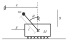
\includegraphics[scale=.8]{figures/mechanicalDrawing}
  \caption{Mechanical drawing of the system, where $\theta$ is the angle of the pendulum, $x$ is the position of the center of the cart along the rail, $F$ is the applied force and $g$ is the gravitational acceleration. It is indicated that friction is modeled between cart and rail as well as in the pendulum joint.}
  \label{fig:mechanicalDrawing}
\end{figure}
The hight of the center of the cart is $l$ such that the pendulum mass center is positioned at zero hight at rest. It is assumed that the pendulum rod is rigid and massless and that the pendulum weights are a point mass at the geometrical center of the weights.\\
The motor torque is given by direct relation to the armature current by the motor constant, $\tau_m = k_\tau i_a $, such that,
\begin{flalign}
F &= \tfrac{1}{r} k_\tau i_a       & \unit{N}  
\label{eq:motorForce}
\end{flalign}
%
It is well known that the potential energy, $U$, and the kinetic energy, $T$, are given by, \cite{RWisniewski}
\begin{flalign}
    U &= mgl( 1 + \cos \theta )   &  \unit{J}  \\
    T &= \frac{1}{2} ( M + m ) \dot{x}^2 - m \dot{x} l \cos \theta \dot{\theta} + \frac{1}{2} m l^2 \dot{\theta}^2 \ \ \ , & \unit{J}
  \label{eq:generalizedPotentialAndKinetic}
\end{flalign}
and that, by use of, \cite{RWisniewski}
\begin{flalign}
  \frac{d}{dt}  \frac{\partial \cal{L}}{\partial \vec{\dot{q}}} - \frac{\partial \cal{L}}{\partial \vec{q}}  &=  \vec{Q} \ \ \ , &
  \label{eq:energyMethodWith external forces}
\end{flalign}
where $\vec{q}=[ \theta\ \ x ]^{\mathrm{T}}$, $\vec{Q} = [\ -b_{p,v} \dot{\theta} - \tanh(\text{k}_\text{tanh}\dot{\theta}) b_{p,c}\ \ \ \ \tfrac{1}{r} k_\tau i_a - b_{c,v} \dot{x} - \tanh(\text{k}_\text{tanh}\dot{x}) b_{c,c}\ ]^{\mathrm{T}}$ and $\cal{L}$ $ = T-U$, the dynamics of the system are found,
\begin{flalign}
    m l^2 \ddot{\theta} - m l \cos \theta \ddot{x} - m g l \sin \theta  &= -b_{p,v} \dot{\theta} - \tanh(\text{k}_\text{tanh}\dot{\theta}) b_{p,c} &  \unit{N \cdot m}  \\
    ( M + m )\ddot{x} + m l \sin \theta \dot{\theta}^2 - m l \cos \theta \ddot{\theta}  &=  \tfrac{1}{r} k_\tau i_a - b_{c,v} \dot{x} - \tanh(\text{k}_\text{tanh}\dot{x}) b_{c,c} \ \ \ , &   \unit{N}
  \label{eq:energyDerivedDynamicEquations}
\end{flalign}
where $\text{k}_\text{tanh}=250$ to approximate a sign-function using tanh.


%---------- Chapter 3 ---------------------------------------- Swing-Up
\chapter{Swing-Up Design}\label{sec:swing-upDesign}
In this chapter a swing-up controller is designed based on \cite{kjAastrom}. The pendulum is started at rest, $\theta = \pi$, angle convention is specified in \autoref{fig:mechanicalDrawing}. The idea of the swing-up controller is to increase the mechanical energy in the system until it matches that of the desired end state, which is the upright position at rest, that is, $\theta = 0$ and $\dot{\theta} = 0$. The minimum energy in the system is the starting position at rest, which is considered to be zero as mentioned in the \textit{Model} \autoref{sec:model}. So the target energy is $E_{\mathrm{eq}} = 2 m g l$, that is, the potential energy of the pendulum in the unstable equilibrium.

Consider the pendulum dynamics from \autoref{eq:energyDerivedDynamicEquation1},
\begin{flalign}
&& J \ddot{\theta} - m l \cos \theta \ddot{x}_c - m g l \sin \theta  &= 0 \ \ \ , &  \unit{N \cdot m}   \label{eq:pendulumDynamics}
\end{flalign}
where $J = m l^2$ is the inertia and the pendulum friction is assumed to be zero. This equation captures the behavior of the pendulum corresponding to some acceleration $\ddot{x}_c$ at the pivot point. This acceleration is viewed as the control input for now. The force needed to achieve this acceleration is considered in the end of the design. It is further convenient to describe the energy of the pendulum with the coordinate frame fixed at its pivot point, see \autoref{fig:fixedCooredinateSystem}.
%
\begin{figure}[H]
  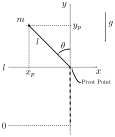
\includegraphics[width=.3\textwidth]{figures/fixedCooredinateSystem}
  \caption{The energy used in the swing-up controller is described using this convention, where the coordinate frame is fixed at the pivot point of the pendulum. The zero reference is placed as before s.t. all energies are positive.}
  \label{fig:fixedCooredinateSystem}
\end{figure}
%
From \autoref{fig:fixedCooredinateSystem}, the conversion from excessive to generalized coordinates is given by,
\begin{flalign}
&& x_p  &= -l \sin \theta   \ \ \ ,\ \ \ y_p = l(\cos \theta + 1)  \ \ \ ,\ \ \ \dot{x}_p = -l \cos \theta \dot{\theta}  \ \ \ ,\ \ \ \dot{y}_p = -l \sin \theta \dot{\theta}  \ \ \ . &&     \label{eq:cooredinateConvertFixed}
\end{flalign}
The mechanical energy in this coordinate frame is then,
\begin{flalign}
&& E_p &= m g y_p + \tfrac{1}{2} m \dot{x}_p^2 + \tfrac{1}{2} m \dot{y}_p^2  &  \unit{J}   \label{eq:pendulumEnergy1} \\
&& E_p &= m g l (\cos \theta +1) + \tfrac{1}{2} m (-l \cos \theta \dot{\theta})^2 + \tfrac{1}{2} m (-l \sin \theta \dot{\theta})^2  &  \unit{J}   \label{eq:pendulumEnergy2} \\
&& E_p &= m g l (\cos \theta +1) + \tfrac{1}{2} J (\cos^2 \theta  + \sin^2 \theta )\dot{\theta}^2  &  \unit{J}   \label{eq:pendulumEnergy3} \\
&& E_p &= \tfrac{1}{2} J \dot{\theta}^2 + m g l (\cos \theta +1) \ \ \ . &  \unit{J}   \label{eq:pendulumEnergy4}
\end{flalign}
%
A Lyapunov function candidate is proposed,
\begin{flalign}
&& V &= \tfrac{1}{2} E_\Delta ^2 \ \ \ ,  \hspace{5cm}  &&&  \label{eq:lyapunovCandidate} 
\end{flalign}
where $E_\Delta$ is the difference in energy in relation to the unstable equilibrium,
%
\begin{flalign}
&& E_\Delta &= E_p  - E_{\mathrm{eq}} &  \unit{J}   \label{eq:energyDelta1} \\
&& E_\Delta &= \tfrac{1}{2} J \dot{\theta}^2 + m g l (\cos \theta +1) - 2 m g l &  \unit{J}   \label{eq:energyDelta2} \\
&& E_\Delta &= \tfrac{1}{2} J \dot{\theta}^2 + m g l (\cos \theta -1)   \ \ \ .  & \unit{J} \label{eq:energyDelta3}
\end{flalign}
%
The derivative of $E_\Delta$ from \autoref{eq:energyDelta3} along the system \autoref{eq:pendulumDynamics} is found to,
\begin{flalign}
&& \dot{E}_\Delta &= J \dot{\theta} \ddot{\theta} - m g l \sin \theta \dot{\theta}  &&&   \label{eq:energyDeltaDerivative1} \\
&& \dot{E}_\Delta &= \dot{\theta} ( m l \cos \theta \ddot{x}_c + m g l \sin \theta )  - m g l \sin \theta \dot{\theta}    &&&   \label{eq:energyDeltaDerivative2} \\
&& \dot{E}_\Delta &=  m l \cos \theta \dot{\theta} \ddot{x}_c \ \ \ .   &&&   \label{eq:energyDeltaDerivative3}
\end{flalign}
The Lyapunov function candidate, \autoref{eq:lyapunovCandidate}, is continuously differentiable in the entire $\mathbb{R} ^2$ \fxnote{brush up on stability criteries}. Its derivative is evaluated to find a stabilizing controller,
%
\begin{flalign}
&& \dot{V} &= E_\Delta \dot{E}_\Delta   \hspace{3cm}  &&&  \label{eq:lyapunovDerivative1}  \\
&& \dot{V} &= E_\Delta m l \cos \theta \dot{\theta} \ddot{x}_c  \leq 0  \ \ \ .  \hspace{3cm}  &&&  \label{eq:lyapunovDerivative2} 
\end{flalign}
%
The acceleration, $\ddot{x}_c$, is then designed to satisfy the stability criterion in \autoref{eq:lyapunovDerivative2},
\begin{flalign}
&& \dot{V} &= m l E_\Delta \cos \theta \dot{\theta} (-E_\Delta \cos \theta \dot{\theta})     \hspace{2cm}  &&&  \label{eq:lyapunovDerivativeControlled1} \\
&& \dot{V} &= -m l (E_\Delta \cos \theta \dot{\theta})^2  \leq 0  \ \ \ ,  \hspace{2cm}  &&&  \label{eq:lyapunovDerivativeControlled2} 
\end{flalign}
further a tuning parameter, $k>0$, is introduced such that the control law for acceleration of the pivot point is,
\begin{flalign}
&& \ddot{x}_c &= -k E_\Delta \cos \theta \dot{\theta}  \ \ \ .  \hspace{4cm}  &&&  \label{eq:accControlLaw} 
\end{flalign}





%---------- Chapter 4 ---------------------------------------- Stabilization
\chapter{Stabilization}
In this section the idea is to stabilize the pendulum in the unstable equilibrium. Ultimately this controller should be able to take over from the swing-up controller when some minimum catch angle is reached.\\
A sliding mode control strategy is employed to accomplish these goals. The design is based on \cite{HKKhalil}.\\
Firstly, the model of the system, from \autoref{eq:nonlinearStateSpace}, is considered in following form,
\begin{align}
  \begin{bmatrix}
    \dot{x}_1 \\
    \dot{x}_2 \\
    \dot{x}_3 \\
    \dot{x}_4
  \end{bmatrix}
  &=
  \underbrace{
    \begin{bmatrix}
      x_3 \\
      x_4 \\
      \vec{M}^{-1}(x_1) ( - \vec{C}(x_1,x_3) - \vec{B}(x_3,x_4) - \vec{G}(x_1) )
    \end{bmatrix}
  }_{\vec{f}(\vec{x})}
  +
  \underbrace{ 
    \begin{bmatrix}
      0 \\
      0 \\
      \vec{M}^{-1}(x_1) \vec{F} 
    \end{bmatrix}
  }_{\vec{g}(\vec{x}) u}
  \label{eq:nonlinearStateSpace2} \ \ \ ,
\end{align}
where
\begin{align}
  \vec{M}^{-1}
  &=
  \begin{bmatrix}
    \frac{(M + m)}{l^2 m ( M + m - m \cos^2 x_1 )}  &  \frac{\cos x_1}{l (M + m - m \cos^2 x_1)} \\
    \frac{\cos x_1}{l (M + m - m \cos^2 x_1)}       &  \frac{1}{M + m - m \cos^2 x_1}
  \end{bmatrix}  \ \ \ ,
\end{align}
%
and states $ [\ x_1\ \ x_2\ \ x_3\ \ x_4\ ]^\mathrm{T} = [\ \theta\ \ x\ \ \dot{\theta}\ \ \dot{x}\ ]^\mathrm{T} $ and input vector $\vec{F} = [\ 0 \ \ u \ ]^\mathrm{T}$ as before.

In \autoref{eq:nonlinearStateSpace2} the input, $u$, appear in two of the four state equations. To design a sliding mode controller for the system, it is transformed into \textit{regular form}, 
\begin{align}
\dot{\vec{\eta}} &=  \vec{f_a}(\vec{\eta},\xi) \nonumber   \\
\dot{\xi}        &=  f_b(\vec{\eta},\xi) + g_b(\vec{\eta},\xi) u    \ \ \ ,
\label{eq:regularForm}
\end{align}
%
where the input only appears on one state equation.
The transform is then given by,
\begin{align}
  \vec{T}(\vec{x}) &=
  \begin{bmatrix}
    \vec{\eta} \\
    \xi
  \end{bmatrix}
  \ \Rightarrow \ 
  \frac{\partial}{\partial t}\vec{T}(\vec{x})
  =
  \begin{bmatrix}
    \dot{\vec{\eta}} \\
    \dot{\xi}
  \end{bmatrix}
  \ \Rightarrow \ 
  \frac{\partial}{\partial t}\vec{T}(\vec{x})
  =
  \begin{bmatrix}
    \vec{f_a}(\vec{\eta},\xi)         \\
    f_b(\vec{\eta},\xi) + g_b(\vec{\eta},\xi) u
  \end{bmatrix}
   \ \ \ ,
  \label{eq:transformAndDerivative}
\end{align}
further,
\begin{align}
  \frac{\partial \vec{T}}{\partial t} &= \frac{\partial \vec{T}}{\partial \vec{x}}  \dot{\vec{x}} \\
  \begin{bmatrix}
    \vec{f_a}(\vec{\eta},\xi)         \\
    f_b(\vec{\eta},\xi) + g_b(\vec{\eta},\xi) u
  \end{bmatrix}
  &=
  \frac{\partial \vec{T}}{\partial \vec{x}} \vec{f}(\vec{x}) + \frac{\partial \vec{T}}{\partial \vec{x}} \vec{g}(\vec{x}) u
  \ \ \ ,
  \label{eq:transformDerivative}
\end{align}
such that,
\begin{align}
  \frac{\partial \vec{T}}{\partial \vec{x}} \vec{f}(\vec{x})    
  &= 
  \begin{bmatrix}
    \vec{f_a}(\vec{\eta},\xi)       \\
    f_b(\vec{\eta},\xi)
  \end{bmatrix}  \ \ \ \ ,\ \ \ \ 
  \frac{\partial \vec{T}}{\partial \vec{x}} \vec{g}(\vec{x})
  = 
  \begin{bmatrix}
    \vec{0}        \\
    g_b(\vec{\eta},\xi)
  \end{bmatrix}
  \ \ \ .
  \label{eq:transformXDerivative}
\end{align}
\autoref{eq:transformXDerivative} results in the following four equations,
\begin{align}
    \frac{\partial \eta_1}{\partial x_3} g_3 + \frac{\partial \eta_1}{\partial x_4} g_4 &= 0                    \ \ \ \ ,\ \ \ \ % \label{eq:chooseEta1}  \\
    \frac{\partial \eta_2}{\partial x_3} g_3 + \frac{\partial \eta_2}{\partial x_4} g_4 = 0         \nonumber   \\ %\label{eq:chooseEta1Eta2}  \\
    \frac{\partial \eta_3}{\partial x_3} g_3 + \frac{\partial \eta_3}{\partial x_4} g_4 &= 0                    \ \ \ \ ,\ \ \ \ %\label{eq:chooseEta3}  \\
    \frac{\partial \xi   }{\partial x_3} g_3 + \frac{\partial \xi   }{\partial x_4} g_4 = g_b(\vec{\eta},\xi)  \label{eq:chooseEta1Eta2Eta3Xi} 
\ \ \ ,
\end{align}
where,
\begin{align}
  \begin{bmatrix}
    g_3  \\
    g_4
  \end{bmatrix} u = \vec{M}^{-1}(x_1) 
    \begin{bmatrix}
      0  \\
      u
    \end{bmatrix} \ \ \ \Rightarrow \ \ \ \ 
  \begin{cases}
    g_3 = \frac{\cos x_1}{l (M + m - m \cos^2 x1)}\\
    g_4 = \frac{1}{M + m - m \cos^2 x_1 }
  \end{cases}
  \label{eq:g_3_and_4} 
\end{align}
%
The following choice of coordinates to satisfy \autoref{eq:chooseEta1Eta2Eta3Xi} without loss of rank in $\vec{T}$, is based on the transform used for input-output linearization in \cite{HKKhalil}.\\
Choosing output, $h(x) = \theta$ or $h(x) = x$, both results in the relative degree, $\rho = 2$, since the output appears on the second derivatives,
\begin{align}
  \ddot{\theta} &= \dot{x}_3 = f_3 + g_3 u
  \label{eq:thetaRelativeDeg} \\
  \ddot{x} &= \dot{x}_4 = f_4 + g_4 u \ \ \ .
  \label{eq:xRelativeDeg} 
\end{align}
The suggested transform is then,
\begin{align}
  \vec{T}(\vec{x})
  =
  \begin{bmatrix}
    \phi_1(\vec{x})         \\
    \vdots                  \\
    \phi_{n-\rho}(\vec{x})  \\
    h(\vec{x})              \\
    L_f h(\vec{x})          \\
    \vdots                  \\
    L_f^{\rho-1} h(\vec{x})
  \end{bmatrix}
  \ \ \Rightarrow \ \ 
  \begin{bmatrix}
  \eta_1   \\
  \eta_2   \\
  \eta_3   \\
  \xi
  \end{bmatrix}
  =
  \begin{bmatrix}
  \phi_1(\vec{x})   \\
  \phi_2(\vec{x})   \\
  h(\vec{x})        \\
  L_f h(\vec{x})
  \end{bmatrix} \ \ \ ,
  \label{eq:transformPhi} 
\end{align}
%
where $L_f h(\vec{x})$ is the \textit{Lie derivative} of $h(\vec{x})$ along $f(\vec{x})$. This results in two possible transforms, 
\begin{align}
h = \theta \ \ \Rightarrow \ \ 
  \vec{T}_1 =
  \begin{bmatrix}
  \eta_1  \\
  \eta_2  \\
  \eta_3  \\
  \xi
  \end{bmatrix}
  =
  \begin{bmatrix}
  \phi_1  \\
  \phi_2  \\
  x_1     \\
  x_3
  \end{bmatrix} \ \ \ \mathrm{and}\ \ h = x \ \ \Rightarrow \ \
  \vec{T}_2 =
  \begin{bmatrix}
  \eta_1   \\
  \eta_2   \\
  \eta_3   \\
  \xi
  \end{bmatrix}
  =
  \begin{bmatrix}
  \phi_1  \\
  \phi_2  \\
  x_2     \\
  x_4
  \end{bmatrix} \ \ \ ,
\end{align}
leaving $\phi_1$ and $\phi_2$ to be determined. This is done by satisfying,
\begin{align}
\frac{\partial \eta_1}{\partial x_3} g_3 + \frac{\partial \eta_1}{\partial x_4} g_4 &= 0       \label{eq:chooseEta1}  \\
\frac{\partial \eta_2}{\partial x_3} g_3 + \frac{\partial \eta_2}{\partial x_4} g_4 &= 0       \label{eq:chooseEta2}  
\ \ \ .
\end{align}
from \autoref{eq:chooseEta1Eta2Eta3Xi}. For $\vec{T}_1$ the choice $\phi_1 = x_2$ satisfies \autoref{eq:chooseEta1} with no loss of rank in the transform. Conversely for $\vec{T}_2$ the choice $\phi_1 = x_1$ satisfies \autoref{eq:chooseEta1} again with no loss of rank. This leaves $\phi_2$ which, for both transforms, is determined by finding a solution to \autoref{eq:chooseEta2},
\begin{align}
 \frac{\partial \eta_2}{\partial x_3} \frac{\cos x_1}{l (M + m - m \cos^2 x1)} + \frac{\partial \eta_2}{\partial x_4} \frac{1}{M + m - m \cos^2 x_1 } = 0 \ \ \ ,
\end{align}
choosing,
\begin{align}
\frac{\partial \eta_2}{\partial x_4} = \frac{\cos x_1}{l}  \ \ , \ \ \ \frac{\partial \eta_2}{\partial x_3}  = -1 \ \ \ ,
\end{align}
such that,
\begin{align}
\eta_2 =  \frac{\cos x_1}{l} x_4 - x_3 \ \ \ .
\end{align}
%
This results in the following two transform candidates,
\begin{align}
%\begin{bmatrix}
%\eta_1   \\
%\eta_2   \\
%\eta_3   \\
%\xi
%\end{bmatrix} \left.\rule{0cm}{1.7cm}\right\vert\rule{0cm}{1.7cm}_{\substack{\rule{0cm}{1.28cm}\\ h=x_1 }}
\vec{T}_1 =
\begin{bmatrix}
x_2   \\
\frac{\cos x_1}{l} x_4 - x_3  \\
x_1   \\
x_3
\end{bmatrix} \ \ \ \ , \ \ \ \
%\begin{bmatrix}
%\eta_1   \\
%\eta_2   \\
%\eta_3   \\
%\xi
%\end{bmatrix} \left.\rule{0cm}{1.7cm}\right\vert\rule{0cm}{1.7cm}_{\substack{\rule{0cm}{1.28cm}\\ h=x_2 }}
\vec{T}_2
=
\begin{bmatrix}
x_1   \\
\frac{\cos x_1}{l} x_4 - x_3   \\
x_2   \\
x_4
\end{bmatrix} \ \ \ .
\end{align}
%
To choose a transform the following is considered.\\
A continuously differentiable map, $\vec{T}$, with a continuously differentiable inverse, $\vec{T}^{-1}$, is known as a diffeomorphism. Further, $\vec{T}$ is a global diffeomorphism iff its Jacobian is nonsingular for all $\vec{x} \in \mathbb{R}^n$ and $\lim_{||\vec{x}||\rightarrow \infty}||\vec{T}(\vec{x})|| = \infty$ , \cite{HKKhalil}.\\
The Jacobian of each transform is computed,
\begin{align}
\vec{J}_1 = \frac{\partial \vec{T}_1(\vec{x})}{\partial \vec{x}}
&=
\begin{bmatrix}
  0                       & 1 &  0 & 0                  \\
  -\frac{\sin x_1}{l} x_4 & 0 & -1 & \frac{\cos x_1}{l} \\
  1                       & 0 &  0 & 0                  \\
  0                       & 0 &  1 & 0
\end{bmatrix}  \label{eq:transform_h_x1} \\
\vec{J}_2 = \frac{\partial \vec{T}_2(\vec{x})}{\partial \vec{x}}
&=
\begin{bmatrix}
  1                       & 0 &  0 & 0                  \\
  -\frac{\sin x_1}{l} x_4 & 0 & -1 & \frac{\cos x_1}{l} \\
  0                       & 1 &  0 & 0                  \\
  0                       & 0 &  0 & 1
\end{bmatrix} \ \ \ . \label{eq:transform_h_x2}
\end{align}
To check for singularity the determinant is found for the two Jacobian matrices. In the case of \autoref{eq:transform_h_x1}, $\det(\vec{J}_1) = -\cos x_1/l$, so if $\cos x_1 = 0$ the Jacobian becomes singular. This only happens when the pendulum is horizontal which is outside the operating range of a stabilizing controller. However, for \autoref{eq:transform_h_x2}, $\det(\vec{J}_2) = 1$, and so, the Jacobian is nonsingular for all $\vec{x} \in \mathbb{R}^4$. Further, $\lim_{||\vec{x}||\rightarrow \infty}||\vec{T}(\vec{x})|| = \infty$ so,
\begin{align}
  \vec{T}
  = 
  \begin{bmatrix}
  \eta_1   \\
  \eta_2   \\
  \eta_3   \\
  \xi
  \end{bmatrix}
  =
  \begin{bmatrix}
  x_1   \\
  \frac{\cos x_1}{l} x_4 - x_3  \\
  x_2   \\
  x_4
  \end{bmatrix} \ \ \ , \label{eq:transform}
\end{align}
is a global diffeomorphism and therefore chosen as the final system transform, with the inverse given by,
\begin{align}
  \vec{T}^{-1} = 
  \begin{bmatrix}
    x_1  \\
    x_2  \\
    x_3  \\
    x_4
  \end{bmatrix}
  =
  \begin{bmatrix}
  \eta_1   \\
  \eta_3   \\
  \frac{\cos \eta_1}{l} \xi - \eta_2  \\
  \xi
  \end{bmatrix} \ \ \ .
  \label{eq:inverseTransform}
\end{align}
%
The derivative of the transform, \autoref{eq:transform}, along the trajectories of the system is,
\begin{align}
  \begin{bmatrix}
    \dot{\eta}_1   \\
    \dot{\eta}_2   \\
    \dot{\eta}_3   \\
    \dot{\xi}
  \end{bmatrix}
  &=
  \begin{bmatrix}
    \dot{x}_1   \\
    \frac{-\sin x_1}{l}\dot{x}_1 x_4 + \frac{\cos x_1}{l} \dot{x}_4 - \dot{x}_3  \\
    \dot{x}_2   \\
    \dot{x}_4
  \end{bmatrix} \label{eq:transform_dt} \\
  %
  %
  %
  \begin{bmatrix}
  \dot{\eta}_1   \\
  \dot{\eta}_2   \\
  \dot{\eta}_3   \\
  \dot{\xi}
  \end{bmatrix} 
  &=
  \begin{bmatrix}
    x_3    \\
    \frac{-\sin x_1}{l} x_3 x_4 + \frac{\cos x_1}{l} f_4(\vec{x}) + \frac{\cos x_1}{l} g_4(\vec{x}) u  - f_3(\vec{x}) - g_3(\vec{x}) u \\
    x_4    \\ 
    f_4(\vec{x}) + g_4(\vec{x}) u 
  \end{bmatrix} \ \ \ , \label{eq:transform_dt_alongTraj}
\end{align}
%
from which the regular form is obtained by rearranging and using the inverse transform,
\begin{align}
\begin{bmatrix}
  \dot{\eta}_1   \\
  \dot{\eta}_2   \\
  \dot{\eta}_3   \\  %these are dotted lines, yea, that's LaTeX for ya, go figure..
  %\begin{picture} (0,0)(0,0) \multiput(-2,14)(4,0){3}{\line(2,0){2}} \end{picture}
  \dot{\xi}
  \end{bmatrix} 
  &=
  \overbrace{
    \underbrace{
      \begin{bmatrix}
      \frac{\cos \eta_1}{l} \xi - \eta_2    \\
      %\frac{l \sin x1}{\cos^2 x_1} x_3^2 +  \tfrac{l}{\cos x_1} f_1(\vec{x})  - f_2(\vec{x}) \\ 
      \frac{-\sin \eta_1}{l} (\frac{\cos \eta_1}{l} \xi - \eta_2) \xi + \frac{\cos \eta_1}{l} f_4(\vec{\eta},\xi) - f_3(\vec{\eta},\xi) \\
      \xi    \\ %these are dotted lines, yea, that's LaTeX for ya, go figure..
      \begin{picture} (0,0)(0,0) \multiput(-95,14)(4,0){57}{\line(2,0){2}} \end{picture}
      f_4(\vec{\eta},\xi) 
      \end{bmatrix}
    }_{f_b} }^{f_a}
  +
  \underbrace{
    \begin{bmatrix}
    0    \\
    0    \\
    0    \\  %these are dotted lines, yea, that's LaTeX for ya, go figure..
    \begin{picture} (0,0)(0,0) \multiput(0,14)(4,0){10}{\line(2,0){2}} \end{picture}
    g_4(\vec{\eta},\xi)
    \end{bmatrix}
  }_{g_b} u  \ \ \ ,
  \label{eq:regularFormMatrix}
\end{align}
where,
\begingroup\makeatletter\def\f@size{10}\check@mathfonts
\def\maketag@@@#1{\hbox{\m@th\normalsize\normalfont#1}}%
\begin{align}
f_3(\vec{\eta},\xi) &= \frac{1}{ l^2 m (M + m - m \cos^2 \eta_1) }
\left[
(M + m) b_{p,v} \left(\eta_2 - \frac{\cos \eta_1 \xi}{l}\right) + \right. \nonumber \\
&+ (M + m) b_{p,c} \tanh\left(\mathrm{k}_{\mathrm{tanh}} \left(\eta_2 - \frac{ \cos \eta_1 \xi}{l}\right)\right) + m^2 g l \sin \eta_1 - b_{c,c} m l \tanh\left(\mathrm{k}_{\mathrm{tanh}} \xi\right) \cos \eta_1 - \nonumber \\
&- \left. m^2 l^2 \cos \eta_1 \sin \eta_1 \left(\eta_2 - \frac{\xi \cos \eta_1}{l}\right)^2 + M g l m \sin \eta_1 - b_{c,v} m l \xi \cos \eta_1
\right] \\
%
%
f_4(\vec{\eta},\xi) &= -\frac{1}{ l (M + m - m \cos^2 \eta_1) } \left[   b_{c,v} l \xi - b_{p,v} \cos \eta_1 \left(\eta_2 - \frac{\cos \eta_1 \xi}{l}\right) + b_{c,c} l \tanh\left(\mathrm{k}_{\mathrm{tanh}} \xi\right) - \right. \nonumber \\
&- b_{p,c} \tanh\left(\mathrm{k}_{\mathrm{tanh}} \left(\eta_2 - \frac{ \cos \eta_1 \xi}{l}\right)\right) \cos \eta_1 + \nonumber \\
&+ \left. l^2 m \sin \eta_1 \left(\eta_2 - \frac{\xi \cos \eta_1}{l}\right)^2 - m g l \cos \eta_1 \sin \eta_1  \right] \\
%
%
g_4(\vec{\eta},\xi) &= \frac{1}{M + m - m \cos^2 \eta_1 }
\ \ \ .
\label{eq:f3f4g4} \\ \nonumber
\end{align}
\endgroup \vspace{-44pt}

%
%
%
%f3 = \frac{ M b_{p,v} (\eta_2 - \frac{\xi \cos \eta_1}{l}) + b_{p,v} m (\eta_2 - \frac{\xi \cos \eta_1}{l}) + M b_{p,c} \tanh(k_{\mathrm{tanh}} (\eta_2 - \frac{\xi \cos \eta_1}{l})) + b_{p,c} m \tanh(k_{\mathrm{tanh}} (\eta_2 - \frac{\xi \cos \eta_1}{l})) + g l m^2 \sin \eta_1 - b_{c,c} l m \tanh(k_{\mathrm{tanh}} \xi) \cos \eta_1 - l^2 m^2 \cos \eta_1 \sin \eta_1 (\eta_2 - \frac{\xi \cos \eta_1}{l})^2 + M g l m \sin \eta_1 - b_{c,v} l m \xi \cos \eta_1 }{ l^2 m (M + m - m \cos^2 \eta_1) }
%
%
%
%f4 = -\frac{1}{ l (M + m - m \cos^2 \eta_1) } \left[   b_{c,v} l \xi - b_{p,v} \cos \eta_1 \left(\eta_2 - \frac{\cos \eta_1 \xi}{l}\right) + b_{c,c} l \tanh\left(\mathrm{k}_{\mathrm{tanh}} \xi\right) - b_{p,c} \tanh\left(\mathrm{k}_{\mathrm{tanh}} \left(\eta_2 - \frac{ \cos \eta_1 \xi}{l}\right)\right) \cos \eta_1 + l^2 m \sin \eta_1 \left(\eta_2 - \frac{\xi \cos \eta_1}{l}\right)^2 - m g l \cos \eta_1 \sin \eta_1  \right]
%
%
\fxnote{Is this too much?}


%\begin{align}
%s &=   \xi - \phi(\vec{\eta}) = 0     \ \ \ ,
%\end{align}
%design $\phi(\vec{\eta})$
%
%if $s = 0$ then $\xi = \phi(\vec{\eta})$, that is, the reduced-order system,
%\begin{align}
%  \vec{\dot{\eta}} &=  f_a(\vec{\eta},\phi(\vec{\eta}))     \ \ \ ,
%  \label{eq:asymStabOrigReducedOrder}
%\end{align}
%is asymptotically stable in the origin.
%
%linearization of reduced-order system,
%%
%\begin{align}
%A &= \frac{\partial \vec{\dot{\eta}}}{\partial \vec{\eta}} \whereThree{\vec{\eta}=\vec{0}\ \ \ \ }{\xi=0\ \ \ \ }{\text{k}_\text{tanh}=1} \ 
%=
%\begin{bmatrix}
%0 & -1                  & 0 \\
%0 & \frac{g_{p,c}}{l m} & g \\
%0 & 0                   & 0 
%\end{bmatrix}   \ \ \ , \ \ \
%B = \frac{\partial \vec{\dot{\eta}}}{\partial \xi} \whereThree{\vec{\eta}=\vec{0}\ \ \ \ }{\xi=0\ \ \ \ }{\text{k}_\text{tanh}=1} \ 
%=
%\begin{bmatrix}
%l  \\
%\frac{-b_{p,v}-b_{p,c}}{l m}  \\
%1  
%\end{bmatrix}   \ \ \ ,
%\label{eq:linearReducedOrder_A}
%\end{align}
%
%stabilize reduced order system by,
%\begin{align}
%\phi(\vec{\eta}) &=   - \vec{k} \vec{\eta}  \ \ \ ,
%\end{align}
%
%design $u$ to bring $s$ to zero.\\
%Lyapunov function candidate, $V = \frac{1}{2}s^2$,
%derivative along trajectories of system
%\begin{align}
%\dot{V} &= s\dot{s} \\
%\dot{V} &= s ( \dot{\xi} + \vec{k}\vec{\dot{\eta}}  ) \\
%\dot{V} &= s ( f_b(\vec{\eta},\xi) + g_b(\vec{\eta},\xi) u +\vec{k}f_a(\vec{\eta},\xi) )  \\
%\dot{V} &= (\vec{k}f_a +  f_b) s + g_b s u \\
%\dot{V} &= g_b s (\vec{k}f_a  +  f_b) g_b^{-1} + g_b s u   \\
%\dot{V} &\leq g_b |s| \left|\vec{k}f_a g_b^{-1} +  f_b \right| + g_b s u  \ \ \ .
%\label{eq:lyapunov}
%\end{align}
%
%using $|s| = \text{sgn}(s) s$ and introducing tuning parameter $\beta_0$ to design $u$,
%\begin{align}
%u = -\text{sgn}(s)\beta (\vec{\eta},\xi) g_b^{-1}(\vec{\eta},\xi) \ \ \ \ \mathrm{where}, \ \ \ \beta(\vec{\eta},\xi)  &= \varrho(\vec{\eta},\xi) + \beta_0 \\
%\mathrm{and}, \ \ \  \varrho(\vec{\eta},\xi) &= \left|\vec{k}f_a  +  f_b \right| \ \ \ .
%\label{eq:ssControlBeta0}
%\end{align}
%s.t.
%\begin{align}
%\dot{V} &\leq g_b |s| \left|\vec{k}f_a +  f_b \right|  g_b^{-1} - g_b\  \mathrm{sgn}(s) s \left|\vec{k}f_a  +  f_b + \beta_0 \right| g_b^{-1}
%\label{eq:lyapunov2}
%\end{align}
%
%
%sign-function discontinuity\\
%sat-function used
%\begin{align}
%\text{sat}\left( \tfrac{s}{\varepsilon} \right) &=
%\begin{cases}
%\ \ \frac{s}{\varepsilon},                           & \ \text{if} \ | \frac{s}{\varepsilon} | \leq 1 \\
%\ \ \text{sgn}\left( \tfrac{s}{\varepsilon} \right), & \ \text{if} \ | \frac{s}{\varepsilon} |  >   1 \ \ \ ,
%\end{cases}
%\label{eq:satuationFunction2}
%\end{align}
%where $\frac{1}{\varepsilon}$ slope
%\begin{align}
%u &= -\text{sat}(\tfrac{s}{\varepsilon})\beta (\vec{\eta},\xi)  g_b^{-1}(\vec{\eta},\xi)  \ \ \ .
%\label{eq:ssControlSat}
%\end{align}
%%



%---------- Chapter 5 ---------------------------------------- Implementation
\chapter{Implementation}
\fxnote{Top for implementation}


\section{Parameter Estimation}
\fxnote{Top for parameter estimation}

\subsection{Cart Friction and Mass}
\fxnote{Write about cart and mass friction}

\subsection{Pendulum Friction}
\fxnote{Write about pendulum friction}



\section{FIR Filter Design}
\fxnote{Write about FIR filter for swing-up}

%---------- Chapter 6 ---------------------------------------- Results
\chapter{Results}
Here the results of the implemented control strategies developed in \textit{Part 1} are presented. Firstly, the swing-up controller is approaching a heteroclinic orbit after seven swings, see \autoref{fig:theta_swing_p00} and \ref{fig:x_swing_p00}, same as achieved in simulation when accounting for actuation limitations.
%ADDITIONAL PLOTS AVAILABLE
%
%thetaDot_swing_p00
%xDot_swing_p00
%thetaDotBiasZoom_swing_p00
%
\begin{figure}[H]
  \hspace{1cm}
  \captionbox
  {
    The swing-up controller approaches the equilibrium and almost reaches the heteroclinic orbit.
    \label{fig:theta_swing_p00}
  }
  {
    \hspace{-1cm}
    \includegraphics[width=.39\textwidth]{figures/theta_swing_p00}
  }
  \hspace{20pt}
  \captionbox 
  {
    Though the cart oscillates more than in the simulation, it stays around zero and within the rail limits during the swing-up sequence.
    \label{fig:x_swing_p00}
  }
  {
    \hspace{-1cm}
    \includegraphics[width=.4\textwidth]{figures/x_swing_p00}
  }  
\end{figure}
%
The controller does fall slightly short of reaching the heteroclinic orbit which is also seen in \autoref{fig:phase_swing_p00}. The energy reference in \autoref{fig:Edelta_swing_p00} reaches zero near the equilibrium points, but must be very slightly below zero when the angular velocity is zero, as otherwise the pendulum would reach equilibrium exactly.
\begin{figure}[H]
  \hspace{1cm}
  \captionbox
  {
    From the test in \autoref{fig:theta_swing_p00} and \ref{fig:x_swing_p00} the energy reference is reached.
    \label{fig:Edelta_swing_p00}
  }
  {
    \hspace{-1cm}
    \includegraphics[width=.4\textwidth]{figures/Edelta_swing_p00}
  }
  \hspace{20pt}
  \captionbox 
  {
    The pendulum almost reaches a heteroclinic orbit.
    \label{fig:phase_swing_p00}
  }
  {
    \hspace{-1cm}
    \includegraphics[width=.364\textwidth]{figures/phase_swing_p00}
  }  
\end{figure}
%
%\begin{figure}[H]
%  \includegraphics[width=.42\textwidth]{figures/ia_swing_p00}
%  \caption{ ia swing p00 }
%  \label{fig:ia_swing_p00}
%\end{figure}
%
It is possible to gain closer proximity to the equilibrium point by increasing the energy reference. In \autoref{fig:theta_swing_p08} and \ref{fig:x_swing_p08} the energy reference is increased by \SI{0.08}{J} to reach heteroclinic orbit.
%
%ADDITIONAL PLOTS AVAILABLE
%
%thetaDot_swing_p08
%xDot_swing_p08
%thetaDotBiasZoom_swing_p08
%
\begin{figure}[H]
  \hspace{1cm}
  \captionbox
  {
    The swing-up controller approaches the equilibrium and eventually reaches the heteroclinic orbit.
    \label{fig:theta_swing_p08}
  }
  {
    \hspace{-1cm}
    \includegraphics[width=.395\textwidth]{figures/theta_swing_p08}
  }
  \hspace{20pt}
  \captionbox 
  {
    The cart does not approach zero position as much as it did in simulation. It does however stay within the constraints of the physical system, which is the main objective of the added position control for the swing-up sequence.
    \label{fig:x_swing_p08}
  }
  {
    \hspace{-1cm}
    \includegraphics[width=.4\textwidth]{figures/x_swing_p08}
  }  
\end{figure}
In \autoref{fig:Edelta_swing_p08} the energy reference is slightly lifted causing a near perfect heteroclinic orbit in \autoref{fig:phase_swing_p08}.
\begin{figure}[H]
  \hspace{1cm}
  \captionbox
  {
    From the test in \autoref{fig:theta_swing_p08} and \ref{fig:x_swing_p08} where the energy reference is raised by \SI{0.08}{J} to get closer to the equilibrium point.
    \label{fig:Edelta_swing_p08}
  }
  {
    \hspace{-1cm}
    \includegraphics[width=.4\textwidth]{figures/Edelta_swing_p08}
  }
  \hspace{20pt}
  \captionbox 
  {
    Near perfect heteroclinic orbit is reached due to the slight increase of the energy reference.
    \label{fig:phase_swing_p08}
  }
  {
    \hspace{-1cm}
    \includegraphics[width=.364\textwidth]{figures/phase_swing_p08}
  }  
\end{figure}
If the model and friction compensation was ideal, no energy offset would be needed, so if a high value was needed to approach equilibrium it might be worth to revisit this part of the design process.\\
%
\autoref{fig:ia_swing_p08} shows the armature current of the motor used to achieve the swing-up behavior with the added energy reference. Though some peaks are present in the current signal, the RMS value does not exceed the continuous current specification of the motor for extended periods of time.
\begin{figure}[H]
  \includegraphics[width=.42\textwidth]{figures/ia_swing_p08}
  \caption{The RMS of the armature current is withing respectable levels of the specified contentious current limit of the motor.}
  \label{fig:ia_swing_p08}
\end{figure}
%
A test of the implemented sliding mode controller is seen in \autoref{fig:theta_slide} and \ref{fig:x_slide} where the angle reaches zero.
%ADDITIONAL PLOTS AVAILABLE
%
%thetaDot_slide
%xDot_slide
%thetaDotBiasZoom_slide
\begin{figure}[H]
  \hspace{1cm}
  \captionbox
  {
    Test of sliding mode controller starting at zero. The controller is subjected to two disturbances after which it rebalances successfully bringing the angle back to zero.
    \label{fig:theta_slide}
  }
  {
    \hspace{-1cm}
    \includegraphics[width=.4\textwidth]{figures/theta_slide}
  }
  \hspace{20pt}
  \captionbox 
  {
    The cart returns approaches zero once the pendulum is rebalanced.
    \label{fig:x_slide}
  }
  {
    \hspace{-1cm}
    \includegraphics[width=.4\textwidth]{figures/x_slide}
  }  
\end{figure}
In the last part, after the \SI{35}{s} mark, an offset in $x$ is observed, this could be contributed to unmodeled friction keeping the control from exceeding the force of friction. The control signal is shown in \autoref{fig:ia_slide} where it does have a constant offset after the \SI{35}{s} mark, supporting the hypothesis. However, the offset is also seen in the other stabilized regions of the test, where the control signal goes to zero. So while the first hypothesis might in part be true, something else is at least contributing to the problem, otherwise the control would still show an offset where the cart position does.
%
\begin{figure}[H]
  \includegraphics[width=.42\textwidth]{figures/ia_slide}
  \caption{The armature current has an offset after \SI{35}{s} which matches an offset in the position, however, around \SI{15}{s} the same offset is seen in position with no offset in armature current.}
  \label{fig:ia_slide}
\end{figure}
%
When testing, an other problem relating to the position of the cart was observed. In \autoref{fig:states_slideEKFproblem} the pendulum is only pushed once in the start of the test. The cart spontaneously diverges from zero position before correcting and re-stabilizing. When this happens, the angular velocity should not increase much, as seen by the FIR filter, which by nature does not introduce bias, however, the EKF shows an increase in angular velocity.
%
\begin{figure}[H]
  \includegraphics[width=.68\textwidth]{figures/states_slideEKFproblem}
  \caption{The system is perturbed about \SI{4}{s} into the test, remaining disturbances are caused by a problem presumed to arise between friction compensation and the EKF.}
  \label{fig:states_slideEKFproblem}
\end{figure}
If the friction compensation is too large, this could cause the cart to move away from equilibrium, and in that event, the EKF which is based on a system model, would get data which does not confine to the model, which might lead to a wrong estimation of the angular velocity, which would then amplify the problem.
%

When finally combining the two control strategies it is advantageous for the catch controller if the swing-up controller is designed to provide a bit of entry velocity at equilibrium. This makes for a more robust swing-up controller, in that, it always reaches the equilibrium in the same number of swings for every test. This means that the swing-up controller would overshoot without a catch controller. However, as the catch controller is enabled close to equilibrium, this helps the sliding mode controller by providing entry velocity at the maximum catch angle.\\
It is further noted that smaller catch angles causes less aggressive actuation of the sliding mode controller. After entering sliding mode the catch angle is increased, such that it stays in sliding mode unless the pendulum exceeds the maximum angle at which sliding mode can successfully re-stabilize the system. When this angle is exceeded, the swing-up controller is enabled and the catch angle is again reduced. As in simulation, a wrapped version of the angle is created such that the pendulum is always at zero when in upright position, this representation is only used by sliding mode.\\
Results of a test of the full implementation of the two controllers is shown in \autoref{fig:theta_swingNslide} and \ref{fig:x_swingNslide}.
%
%ADDITIONAL PLOTS AVAILABLE
%
%thetaDot_swingNslide
%xDot_swingNslide
%phase_swingNslide
%Edelta_swingNslide
\begin{figure}[H]
  \hspace{1cm}
  \captionbox
  {
    Test of the final design of swing-up with the higher energy reference and sliding mode controller successfully catching the pendulum after seven swings.
    \label{fig:theta_swingNslide}
  }
  {
    \hspace{-1cm}
    \includegraphics[width=.384\textwidth]{figures/theta_swingNslide}
  }
  \hspace{20pt}
  \captionbox 
  {
    The cart keeps around zero on the rail, especially after the pendulum angle is controlled to zero.
    \label{fig:x_swingNslide}
  }
  {
    \hspace{-1cm}
    \includegraphics[width=.4\textwidth]{figures/x_swingNslide}
  }  
\end{figure}
The swing-up controller successfully hands over to sliding mode after seven swings and the sliding mode controller stabilizes the system in zero with some offset in the cart position.
The moving average RMS of the actuation current briefly exceeds the continuous current rating of the motor when sliding mode catches the pendulum. As this is not happening over a prolonged period, it is not thought to be a problem,
\begin{figure}[H]
  \includegraphics[width=.42\textwidth]{figures/ia_swingNslide}
  \caption{Armature current of the finished control system. It only briefly exceeds the motor specifications when the sliding mode controller takes over.}
  \label{fig:ia_swingNslide}
\end{figure}
%
Three energy based swing-up designs were investigated, the sat-based version was chosen, a cart position controller was added and finally a stabilizing sliding mode controller was designed to catch the pendulum in equilibrium. The designs were successfully implemented and tested on the system setup concluding \textit{Part 1} of this thesis.

%%% PART 2 %%%
\part{Twin Pendulum}

%---------- Chapter 1 ---------------------------------------- System and Model
\chapter{System and Model}
The cart pendulum system from \textit{Part 1} is used again. However, here in \textit{Part 2} an additional pendulum is mounted on the cart. The modification is discussed and a model for the changed system is developed in this chapter. The remaining of \textit{Part 2} is concerned with estimating parameters, developing a state estimator and ultimately stabilizing the two pendulums in upright position.

\section{System Addition}


\section{Model}
To model the twin pendulum system, consider the excessive coordinate convention in \autoref{fig:excessiveCoordinatesTwin} along with the generalized coordinates in the mechanical drawing, \autoref{fig:mechanicalDrawingTwin}.
\begin{figure}[H]
  \captionbox
  {
    Twin pendulum system in excessive coordinates.
    \label{fig:excessiveCoordinatesTwin}
  }
  {
    \hspace{-1cm}
    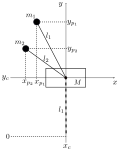
\includegraphics[width=.35\textwidth]{figures/excessiveCoordinatesTwin}
  }
  \hspace{40pt}
  \captionbox
  {
    Mechanical drawing of the system with the added pendulum in generalized coordinates.
    \label{fig:mechanicalDrawingTwin}
  }
  {
    \hspace{-1cm}
    \includegraphics[width=.43\textwidth]{figures/mechanicalDrawingTwin}\vspace{1.2cm}
  }  
\end{figure}
%
The energy method is applied. First the potential and kinetic energies, in therms of excessive coordinates, is found,
\begin{align}
  U &= M g y_c + m_1 g y_{p_1} + m_2 g y_{p_2}  \label{eq:potentialEnergyTwin}  \\
  T &= \tfrac{1}{2} M \dot{x}_c^2 + \tfrac{1}{2} M \dot{y}_c^2 + \tfrac{1}{2} m_1 \dot{x}_{p_1}^2  + \tfrac{1}{2} m_1 \dot{y}_{p_1}^2 + \tfrac{1}{2} m_2 \dot{x}_{p_2}^2 + \tfrac{1}{2} m_2 \dot{y}_{p_2}^2 \label{eq:kineticEnergyTwin} \ \ \ .
\end{align}
%
The excessive coordinates and derivatives thereof are then expressed in therms of the generalized coordinates, using the conventions presented in \autoref{fig:excessiveCoordinatesTwin} and \ref{fig:mechanicalDrawingTwin},
\begin{align}
  \begin{cases}
    x_c &=  x  \\
    y_c &=  l_1  
  \end{cases} &
  \hspace{20pt}
  \begin{cases}
    x_{p_1} =  x   - l_1 \sin \theta_1 \\
    y_{p_1} =  l_1 + l_1 \cos \theta_1
  \end{cases}
  \hspace{10pt}
  \begin{cases}
    x_{p_2} =  x   - l_2 \sin \theta_2 \\
    y_{p_2} =  l_1 + l_2 \cos \theta_2
  \end{cases}
  \label{eq:excessiveToGeneralized} \\
  \begin{cases}
    \dot{x}_c &=  \dot{x}  \\
    \dot{y}_c &=  0  
  \end{cases} &
  \hspace{20pt}
  \begin{cases}
    \dot{x}_{p_1} =  \dot{x} - l_1 \sin \theta_1 \\
    \dot{y}_{p_1} =  -l_1 \sin \theta_1 \dot{\theta}_1
  \end{cases}
  \hspace{10pt}
  \begin{cases}
    \dot{x}_{p_2} = \dot{x} - l_2 \sin \theta_2 \\
    \dot{y}_{p_2} = -l_2 \sin \theta_2 \dot{\theta}_2
  \end{cases}  \ \ \ .
  \label{eq:excessiveToGeneralizedDerivatives}
\end{align}

Inserting \autoref{eq:excessiveToGeneralized} and \ref{eq:excessiveToGeneralizedDerivatives} into the energy equations, \autoref{eq:potentialEnergyTwin} and \ref{eq:kineticEnergyTwin}, yields,
%
\begin{align}
  U &= M g l_1 + m_1 g (l_1 + l_1 \cos \theta_1) + m_2 g (l_1 + l_2 \cos \theta_2)  \label{eq:potentialEnergyTwinGeneralized}  \\
  T &= \tfrac{1}{2} M \dot{x}^2 + \tfrac{1}{2} m_1 (\dot{x} - l_1 \sin \theta_1)^2  + \tfrac{1}{2} m_1 (-l_1 \sin \theta_1 \dot{\theta}_1)^2 + \nonumber \\
    &+ \tfrac{1}{2} m_2 (\dot{x} - l_2 \sin \theta_2)^2 + \tfrac{1}{2} m_2 (-l_2 \sin \theta_2 \dot{\theta}_2)^2 \label{eq:kineticEnergyTwinGeneralized} \ \ \ .
\end{align}
%
Proceeding to compute the Lagrangian,
\begin{align}
  \cal{L} &= T - U   \\ 
%  \cal{L} &= \tfrac{1}{2} M \dot{x}^2 + \tfrac{1}{2} m_1 (\dot{x} - l_1 \sin \theta_1)^2  + \tfrac{1}{2} m_1 (-l_1 \sin \theta_1 \dot{\theta}_1)^2  \\
%          &+ \tfrac{1}{2} m_2 (\dot{x} - l_2 \sin \theta_2)^2 + \tfrac{1}{2} m_2 (-l_2 \sin \theta_2 \dot{\theta}_2)^2 \\
%          &- M g l_1 - m_1 g (l_1 + l_1 \cos \theta_1) - m_2 g (l_1 + l_2 \cos \theta_2)) \\
  \cal{L} &= \tfrac{1}{2} M \dot{x}^2 + \tfrac{1}{2} m_1 ( \dot{x}^2 + l_1^2 \cos ^2 \theta_1 \dot{\theta}_1^2 - 2 \dot{x} l_1 \cos \theta_1 \dot{\theta}_1 ) + \tfrac{1}{2} m_1 l_1^2 \sin ^2 \theta_1 \dot{\theta}_1^2 + \nonumber \\
          &+ \tfrac{1}{2} m_2 ( \dot{x}^2 + l_2^2 \cos ^2 \theta_2 \dot{\theta}_2^2 - 2 \dot{x} l_2 \cos \theta_2 \dot{\theta}_2 ) + \tfrac{1}{2} m_2 l_2^2 \sin ^2 \theta_2 \dot{\theta}_2^2 - \nonumber \\
          &-(M + m_1 + m_2) g l_1 - m_1 g l_1 \cos \theta_1 - m_2 g l_2 \cos \theta_2 \\
  \cal{L} &= \tfrac{1}{2} (M + m_1 + m_2) \dot{x}^2 - ( m_1 l_1 \cos \theta_1 \dot{\theta}_1 + m_2 l_2 \cos \theta_2 \dot{\theta}_2 ) \dot{x} + \nonumber \\
          &+ \tfrac{1}{2} m_1 l_1^2 (\cos^2 \theta_1 + \sin^2 \theta_1)\dot{\theta}_1^2 + \tfrac{1}{2} m_2 l_2^2 (\cos^2 \theta_2 + \sin^2 \theta_2)\dot{\theta}_2^2 - \nonumber \\
          &- (M + m_1 + m_2)g l_1 - m_1 g l_1 \cos \theta_1 - m_2 g l_2 \cos \theta_2  \\
  \cal{L} &= \tfrac{1}{2} (M + m_1 + m_2) \dot{x}^2 - ( m_1 l_1 \cos \theta_1 \dot{\theta}_1 + m_2 l_2 \cos \theta_2 \dot{\theta}_2 ) \dot{x} + \tfrac{1}{2} m_1 l_1^2 \dot{\theta}_1^2 + \nonumber \\
          &+ \tfrac{1}{2} m_2 l_2^2 \dot{\theta}_2^2 - (M + m_1 + m_2)g l_1 - m_1 g l_1 \cos \theta_1 - m_2 g l_2 \cos \theta_2
  \ \ \ , 
  \label{eq:lagrangian}
\end{align}
and finally by using the Lagrange-d’Alembert Principle, \cite{RWisniewski}
\begin{align}
  \frac{d}{dt}  \frac{\partial \cal{L}}{\partial \dot{\vec{q}}} - \frac{\partial \cal{L}}{\partial \vec{q}}  &=  \vec{Q} \ \ \ ,
  \label{eq:energyMethodWithExternalForcesTwin}
\end{align}
\begin{align}
  \vec{q} &= 
  \begin{bmatrix}
    \theta_1    \\
    \theta_2    \\
    x
  \end{bmatrix} \ \ \ , \ \ \ 
  \vec{Q} =
  \begin{bmatrix}
    -b_{p_1,v} \dot{\theta}_1 - \tanh(\text{k}_\text{tanh}\dot{\theta}_1) b_{p_1,c}    \\
    -b_{p_2,v} \dot{\theta}_2 - \tanh(\text{k}_\text{tanh}\dot{\theta}_2) b_{p_2,c}    \\
    u - b_{c,v} \dot{x} - \tanh(\text{k}_\text{tanh}\dot{x}) b_{c,c}
  \end{bmatrix} \ \ \ .
  \label{eq:qAndQ_twin}
\end{align}
%
Note that, as in \textit{Part 1}, the control output is seen as the force on the cart directly, $u = F$, to avoid excessive notation. \autoref{eq:energyMethodWithExternalForcesTwin} is computed for each generalized coordinate starting with the first pendulum angle, $\theta_1$,
\begin{gather}
\frac{d}{dt}  \frac{\partial \cal{L}}{\partial \dot{\theta}_1} - \frac{\partial \cal{L}}{\partial \theta_1}  = Q_1 \\
m_1 l_1 \sin \theta_1 \dot{\theta}_1 \dot{x} - m_1 l_1 \cos \theta_1 \ddot{x} + m_1 l_1^2 \ddot{\theta}_1 - m_1 l_1 \sin \theta_1 \dot{\theta}_1 \dot{x} - m_1 g l_1 \sin \theta_1 = Q_1  \\
- m_1 l_1 \cos \theta_1 \ddot{x} + m_1 l_1^2 \ddot{\theta}_1 - m_1 g l_1 \sin \theta_1 = -b_{p_1,v} \dot{\theta}_1 - \tanh(\text{k}_\text{tanh}\dot{\theta}_1) b_{p_1,c}  \ \ \ ,
\label{eq:theta1Dynamics}
\end{gather}
similarly for the second pendulum angle, $\theta_2$,
\begin{gather}
- m_2 l_2 \cos \theta_2 \ddot{x} + m_2 l_2^2 \ddot{\theta}_2 - m_2 g l_2 \sin \theta_2 = -b_{p_2,v} \dot{\theta}_2 - \tanh(\text{k}_\text{tanh}\dot{\theta}_2) b_{p_2,c}  \ \ \ ,
\label{eq:theta2Dynamics}
\end{gather}
and finally for the cart position, $x$,
\begin{gather}
\frac{d}{dt}  \frac{\partial \cal{L}}{\partial \dot{x}} - \frac{\partial \cal{L}}{\partial x}  = Q_3 \\
(M + m_1 + m_2) \ddot{x} + m_1 l_1 \sin \theta_1 \dot{\theta}_1^2 - m_1 l_1 \cos \theta_1 \ddot{\theta}_1 + \nonumber \\
+ m_2 l_2 \sin \theta_2 \dot{\theta}_2^2 - m_2 l_2 \cos \theta_2 \ddot{\theta}_2 = u - b_{c,v} \dot{x} - \tanh(\text{k}_\text{tanh}\dot{x}) b_{c,c}  \ \ \ .
\label{eq:xDynamics}
\end{gather}
%
The final dynamic equations for the twin pendulum system are then,
%
\begingroup\makeatletter\def\f@size{10}\check@mathfonts
\def\maketag@@@#1{\hbox{\m@th\normalsize\normalfont#1}}%
\begin{gather}
- m_1 l_1 \cos \theta_1 \ddot{x} + m_1 l_1^2 \ddot{\theta}_1 - m_1 g l_1 \sin \theta_1 = Q_1 
\label{eq:theta1Dynamics1} \\
- m_2 l_2 \cos \theta_2 \ddot{x} + m_2 l_2^2 \ddot{\theta}_2 - m_2 g l_2 \sin \theta_2 = Q_2
\label{eq:theta2Dynamics1} \\
(M + m_1 + m_2) \ddot{x} + m_1 l_1 \sin \theta_1 \dot{\theta}_1^2 - m_1 l_1 \cos \theta_1 \ddot{\theta}_1 + m_2 l_2 \sin \theta_2 \dot{\theta}_2^2 - m_2 l_2 \cos \theta_2 \ddot{\theta}_2 = Q_3  \ \ \ , 
\label{eq:xDynamics1} \\ \nonumber
\end{gather}\endgroup \vspace{-44pt}

\fxnote{compare dynamic equations to single pendulum equations.} and arranged in following manner,
%
\begingroup\makeatletter\def\f@size{10}\check@mathfonts
\def\maketag@@@#1{\hbox{\m@th\normalsize\normalfont#1}}%
\begin{align}
  \begin{split}
    &
    \begin{bmatrix}
      m_1 l_1^2              & 0                       &  -m_1 l_1 \cos \theta_1 \\
      0                      & m_2 l_2^2               &  -m_2 l_2 \cos \theta_2\\
      -m_1 l_1 \cos \theta_1 & -m_2 l_2 \cos \theta_2  &  M + m_1 + m_2
    \end{bmatrix}
    \begin{bmatrix}
      \ddot{\theta}_1  \\
      \ddot{\theta}_2  \\
      \ddot{x}
    \end{bmatrix}
    +
    \begin{bmatrix}
    0  \\
    0  \\
    m_1 l_1 \sin \theta_1 \dot{\theta}_1^2 + m_2 l_2 \sin \theta_2 \dot{\theta}_2^2
    \end{bmatrix}
    +   \\
    &+
    \begin{bmatrix}
      -b_{p_1,v} \dot{\theta}_1 - \tanh(\text{k}_\text{tanh}\dot{\theta}_1) b_{p_1,c}    \\
      -b_{p_2,v} \dot{\theta}_2 - \tanh(\text{k}_\text{tanh}\dot{\theta}_2) b_{p_2,c}    \\
      -b_{c,v} \dot{x} - \tanh(\text{k}_\text{tanh}\dot{x}) b_{c,c}
    \end{bmatrix}
    +
    \begin{bmatrix}
      -m_1 g l_1 \sin \theta_1  \\
      -m_2 g l_2 \sin \theta_2  \\
      0
    \end{bmatrix}
    =
    \begin{bmatrix}
      0  \\
      0  \\
      u
    \end{bmatrix} \ \ \ , 
  \end{split}
  \label{eq:theta1Theta2Xdynamics} \\ \nonumber
\end{align}
\endgroup \vspace{-44pt}

the well known general form of an m-link robot is obtained, \cite{MWSpong, LSciavicco}
\begin{align}
\vec{M}(\vec{q})\vec{\ddot{q}} + \vec{C}(\vec{q},\vec{\dot{q}}) + \vec{B}(\vec{\dot{q}}) + \vec{G}(\vec{q}) &= \vec{F} \ \ \ , \hspace{3.3cm}
\end{align}
\begin{where}
  \va{ \vec{M}(\vec{q})  }{is the inertia matrix}                    {}
  \va{ \vec{C}(\vec{q},\vec{\dot{q}})  }{is the Coriolis and centrifugal effects}  {}
  \va{ \vec{B}(\vec{\dot{q}})          }{is the friction}                          {}
  \va{  \vec{G}(\vec{q})               }{is the force due to gravity}              {}
  \va{  \vec{F}                        }{is the input force vector \ \ \ .}        {}
\end{where}

Choosing states $ [\ x_1\ \ x_2\ \ x_3\ x_4\ \ x_5\ \ x_6\ ]^\mathrm{T} = [\ \theta_1\ \ \theta_2\ \ x\ \ \dot{\theta}_1\ \ \dot{\theta}_2\ \ \dot{x}\ ]^\mathrm{T} $ results in the nonlinear state space representation,
%
%\begingroup\makeatletter\def\f@size{10}\check@mathfonts
%\def\maketag@@@#1{\hbox{\m@th\normalsize\normalfont#1}}%
\begin{align}
  \begin{bmatrix}
    \dot{x_1} \\
    \dot{x_2} \\
    \dot{x_3} \\
    \dot{x_4} \\
    \dot{x_5} \\
    \dot{x_6}
  \end{bmatrix}
  &=
  \begin{bmatrix}
    x_4 \\
    x_5 \\
    x_6 \\
    \\
    \vec{M}^{-1}(x_1,x_2) ( \vec{F} - \vec{C}(x_1,x_2,x_4,x_5) - \vec{B}(x_4,x_5,x_6) - \vec{G}(x_1,x_2) ) \\
    \phantom{eq}
  \end{bmatrix}
  \label{eq:nonlinearStateSpaceTwin} \ \ \ . %\\ \nonumber
\end{align}
%\endgroup \vspace{-44pt}
%

















%---------- Chapter 2 ---------------------------------------- Swing-Up
% !TeX root = ../main.tex
%
\chapter{Swing-Up Design}
This chapter contains a swing-up design for the twin pendulum system. As for the cart pendulum system in \textit{Part 1} the design is based on \cite{kjAastrom}. The presented approach is similar to the sat-based energy controller, the final design from \textit{Part 1}. Detailed nonlinear analysis is left out here since this design exploits the same principals as for the final cart pendulum swing-up controller in \textit{Part 1}.\\
Both pendulums are started in $\pi$ at rest and the design is based on the pendulum energies in the coordinate system fixed to the cart, thus reducing the generalized coordinates to,
%
\begingroup\makeatletter\def\f@size{10}\check@mathfonts
\def\maketag@@@#1{\hbox{\m@th\normalsize\normalfont#1}}%
\begin{flalign}
  &
  \begin{cases}
    x_{p_1} =  - l_1 \sin \theta_1 \\
    y_{p_1} =  l_1 + l_1 \cos \theta_1
  \end{cases}
  %\hspace{10pt}
  \begin{cases}
    x_{p_2} =  - l_2 \sin \theta_2 \\
    y_{p_2} =  l_1 + l_2 \cos \theta_2
  \end{cases}
  %\label{eq:excessiveToGeneralized2} \\
  \begin{cases}
    \dot{x}_{p_1} =  - l_1 \cos \theta_1 \dot{\theta}_1 \\
    \dot{y}_{p_1} =  -l_1 \sin \theta_1 \dot{\theta}_1
  \end{cases}% &
  %\hspace{10pt}
  \begin{cases}
    \dot{x}_{p_2} = - l_2 \cos \theta_2 \dot{\theta}_2 \\
    \dot{y}_{p_2} = -l_2 \sin \theta_2 \dot{\theta}_2 \ \ \ \ .
  \end{cases}\hspace{-1cm}
  \label{eq:excessiveToGeneralizedDerivatives2}
  &\\ \nonumber
\end{flalign}\endgroup \vspace{-44pt}

Since the energies of the two pendulums are described in a local coordinate system fixed to the cart, there is no cross-coupling, thus the energies are independent of one another,
%
\begin{align}
  E_{p_1} &= m_1 g y_{p_1} + \tfrac{1}{2} m_1 \dot{x}_{p_1}^2 + \tfrac{1}{2} m_1 \dot{y}_{p_1}^2             \label{eq:pendulum1Energy} \\
  E_{p_2} &= m_2 g y_{p_2} + \tfrac{1}{2} m_2 \dot{x}_{p_2}^2 + \tfrac{1}{2} m_2 \dot{y}_{p_2}^2   \ \ \ ,   \label{eq:pendulum2Energy}
\end{align}
%
and in generalized coordinates,
\begin{align}
  E_{p_1} &= \tfrac{1}{2} J_1 \dot{\theta}_1^2 + m_1 g l_1 (\cos \theta_1 + 1)             \label{eq:pendulum1EnergyGeneralized} \\
  E_{p_2} &= \tfrac{1}{2} J_2 \dot{\theta}_2^2 + m_2 g (l_2 \cos \theta_2 + l_1) \ \ \ ,   \label{eq:pendulum2EnergyGeneralized}
\end{align}
%
where the inertia $J_1 = m_1 l_1^2$ and $J_2 = m_2 l_2^2$ and the energy in equilibrium for each pendulum is,
\begin{align}
  & E_{eq_1} = 2 m_1 g l_1 \ \ \ , \ \ \ \ E_{eq_2} = m_2 g (l1 + l2)   \ \ \ ,    \label{eq:eqEnergyTwin}
\end{align}
%
such that,
\begin{align}
  E_{\Delta_1} &= E_{p_1} - E_{eq_1} = \tfrac{1}{2} J_1 \dot{\theta}_1^2 + m_1 g l_1 (\cos \theta_1 - 1)             \label{eq:pendulum1EnergyError} \\
  E_{\Delta_2} &= E_{p_2} - E_{eq_2} =  \tfrac{1}{2} J_2 \dot{\theta}_2^2 + m_2 g l_2 (\cos \theta_2 - 1) \ \ \ .   \label{eq:pendulum2EnergyError}
\end{align}
%
Choosing the function candidate,
\begin{align}
  V(\theta_1, \theta_2, \dot{\theta}_1, \dot{\theta}_2) &= \tfrac{1}{2} E_{\Delta_1} ^2 + \tfrac{1}{2} E_{\Delta_1} ^2 \ \ \ ,   \label{eq:lyapunovCandidateTwin} 
\end{align}
%
and with the dynamics given by,
\begin{align}
  J \ddot{\theta} &= m_1 l_1 \cos \theta_1 a_c + m_1 g l_1 \sin \theta_1          \label{eq:pendulum1DynamicsTwin} \\
  J \ddot{\theta} &= m_2 l_2 \cos \theta_2 a_c + m_2 g l_2 \sin \theta_2 \ \ \ ,  \label{eq:pendulum2DynamicsTwin}
\end{align}
%
the derivative of $V$ is evaluated along trajectories of the system,
\begin{align}
  \dot{V} &= E_{\Delta_1} \dot{E}_{\Delta_1} + E_{\Delta_2} \dot{E}_{\Delta_2}
  \label{eq:lyapunovDerivativeTwin1} \\ 
  \dot{V} &=
  E_{\Delta_1} ( J_1 \dot{\theta}_1 \ddot{\theta}_1 - m_1 g l_1 \sin \theta_1 \dot{\theta}_1 )  \nonumber \\
  &+
  E_{\Delta_2} ( J_2 \dot{\theta}_2 \ddot{\theta}_2 - m_2 g l_2 \sin \theta_2 \dot{\theta}_2 ) 
  \label{eq:lyapunovDerivativeTwin2} \\
  \dot{V} &= E_{\Delta_1} ( \dot{\theta}_1 ( m_1 l_1 \cos \theta_1 a_c + m_1 g l_1 \sin \theta_1 )  - m_1 g l_1 \sin \theta_1 \dot{\theta}_1 ) \nonumber \\
  &+
  E_{\Delta_2} ( \dot{\theta}_2 ( m_2 l_2 \cos \theta_2 a_c + m_2 g l_2 \sin \theta_2 )  - m_2 g l_2 \sin \theta_2 \dot{\theta}_2 )
  \label{eq:lyapunovDerivativeTwin3} \\
  \dot{V} &= G a_c   \ \ \ ,  \label{eq:lyapunovDerivativeTwin4}
\end{align}
%
where,
\begin{align}
  G &= m_1 l_1 E_{\Delta_1} \cos \theta_1 \dot{\theta}_1 +  m_2 l_2 E_{\Delta_2} \cos \theta_2 \dot{\theta}_2  \ \ \ .  \label{eq:lyapunovDerivativeTwinG}
\end{align}
Following control law for the pivot point acceleration, $a_c$, is chosen such that $\dot{V}$ is negative semi-definite,
\begin{align}
  a_c &= sat( -k G ) \ \ \ ,  \label{eq:twinSwingControl1}
\end{align}
where $k$ is a tuning parameter and,
\begin{align}
  \text{sat}(s) &=
  \begin{cases}
    \ \ s                           & \ \  | s |  \leq a_{max} \\
    \ \ \mathrm{sgn}( s )\ a_{max}  & \ \  | s |  >  a_{max} \ \ \ .
  \end{cases}
  \label{eq:satuationFunctionTwin}
\end{align}
%
This control law exhibits the same properties as the first design in \textit{Part 1}, thus the largest invariant set also contains the stable equilibrium at $\pi$, which is the starting position of the pendulums. For this design, the issue is solved by applying a large current, $i_{max}=$ \SI{4.58}{A}, for \SI{0.1}{s} before initiating the swing-up sequence, thus starting at some initial values for which the control signal is different from zero.\\
The controller for cart position from \textit{Part 1} is used unchanged in this design.
%
\begin{figure}[H]
  \hspace{-10pt}
  \captionbox 
  {
    The mechanical energy for each pendulum approach that of their respective equilibrium points shown here by difference in energy.
    \label{fig:Edelta_twinSwing}
  }
  {
    \hspace{-1cm}
    \includegraphics[width=.448\textwidth]{figures/Edelta_twinSwing}
  }
  \hspace{20pt}
  \captionbox 
  {
    Both pendulums of the twin system successfully reaches their heteroclinic orbit. Notice how the shorter pendulum (red) reaches higher angular velocity at its orbit than the longer pendulum (blue), which makes sense as the shorter pendulum has a higher frequency.
    \label{fig:phase_twinSwing}
  }
  {
    \hspace{-1cm}
    \includegraphics[width=.46\textwidth]{figures/phase_twinSwing}
  }
\end{figure}
%
The design is implemented for simulation, see \autoref{fig:Edelta_twinSwing} and \ref{fig:phase_twinSwing}, effectively driving the energy differences to zero and reaching a heteroclinic orbit for both pendulums. In these simulations the gain is chosen to $k=16$ and \SI{.022}{J} is added to the energy references to reach orbit.
%
%
In \autoref{fig:theta_twinSwing} and \ref{fig:ani_twinSwing} it is seen that though the two pendulums reach their heteroclinic orbits, they do not necessarily reach equilibrium simultaneously. However, using a wrapped version of the angles, same as in \textit{Part 1}, it is possible to catch both pendulums while in opposing equilibrium points. Such a scenario is seen most clearly at the end in \autoref{fig:theta_twinSwing} and \ref{fig:ani_twinSwing} about 11 swings into the simulation.
\begin{figure}[H]
  \hspace{-10pt}
  \captionbox 
  {
    Due to different lengths of the two pendulums the frequencies are different thus the signals drift compared to one another.
    \label{fig:theta_twinSwing}
  }
  {
    \hspace{-1cm}
    \includegraphics[width=.46\textwidth]{figures/theta_twinSwing}
  }
  \hspace{20pt}
  \captionbox 
  {
    The two pendulums meet in upright position but at opposing equilibrium points.
    \label{fig:ani_twinSwing}
  }
  {
    \hspace{-1cm}
    \includegraphics[width=.46\textwidth]{figures/ani_twinSwing}
  }
\end{figure}
%
The control signal used to obtain the behavior in these simulations are shown in \autoref{fig:ia_twinSwing}.
%
\begin{figure}[H]
  \includegraphics[width=.5\textwidth]{figures/ia_twinSwing}
  \caption{The control signal required for the twin pendulum swing-up behavior simulated in this chapter is within the limits of the motor.}
  \label{fig:ia_twinSwing}
\end{figure}
%
\autoref{fig:x_twinSwing} and \ref{fig:xDot_twinSwing} shows that the position control from \textit{Part 1} also works well with the twin pendulum swing-up design.
\begin{figure}[H]
  \hspace{-10pt}
  \captionbox
  {
    The position control design used in \textit{Part 1} also shows good results for the twin pendulum.
    \label{fig:x_twinSwing}
  }
  {
    \hspace{-1cm}
    \includegraphics[width=.4\textwidth]{figures/x_twinSwing}
  }
  \hspace{20pt}
  \captionbox 
  {
    Both states, $x$ and $\dot{x}$, are successfully brought to around zero while still allowing the swing-up controller to maintain orbit.
    \label{fig:xDot_twinSwing}
  }
  {
    \hspace{-1cm}
    \includegraphics[width=.4\textwidth]{figures/xDot_twinSwing}
  }  
\end{figure}
%
%
%\begin{figure}[H]
%  \includegraphics[width=.6\textwidth]{figures/thetaDot_twinSwing}
%  \caption{thetaDotTwinSwing}
%  \label{fig:thetaDot_twinSwing}
%\end{figure}
%\begin{figure}[H]
%  \includegraphics[width=.6\textwidth]{figures/thetaDotDot_twinSwing}
%  \caption{thetaDotDotTwinSwing}
%  \label{fig:thetaDotDot_twinSwing}
%\end{figure}
%\begin{figure}[H]
%  \includegraphics[width=.6\textwidth]{figures/xDotDot_twinSwing}
%  \caption{xDotDotTwinSwing}
%  \label{fig:xDotDot_twinSwing}
%\end{figure}

\fxnote{tail for twin swing-up}

%---------- Chapter 3 ---------------------------------------- Stabilization
% !TeX root = ../main.tex
%
\chapter{Stabilization}
%
%\begin{figure}[H]
%  \hspace{-10pt}
%  \captionbox 
%  {
%    a
%    \label{fig:Edelta_twinSwingAndCatch}
%  }
%  {
%    \hspace{-1cm}
%    \includegraphics[width=.448\textwidth]{figures/Edelta_twinSwingAndCatch}
%  }
%  \hspace{20pt}
%  \captionbox 
%  {
%    a
%    \label{fig:phase_twinSwingAndCatch}
%  }
%  {
%    \hspace{-1cm}
%    \includegraphics[width=.46\textwidth]{figures/phase_twinSwingAndCatch}
%  }
%\end{figure}
%
In this chapter a Linear Quadratic Regulator (LQR) is designed to stabilize the twin pendulum in upright position taking over from the swing-up controller.\\
The nonlinear state space system from \autoref{eq:nonlinearStateSpaceTwin} is linearized,
\begin{align}
  \vec{A} &= \frac{\partial \vec{f(x)}}{\partial \vec{x}} \whereThree{\vec{x}=\vec{0}\ \ \ \ }{u=0\ \ \ \ }{\text{k}_\text{tanh}=1} \ \ \ , \ \ \
  \vec{B} = \frac{\partial \vec{f(x)}}{\partial u}  \whereThree{\vec{x}=\vec{0}\ \ \ \ }{u=0\ \ \ \ }{\text{k}_\text{tanh}=1} \ \ \ ,
  \label{eq:linearTwin_AB}
\end{align}
\begin{align}
  \vec{A} &= 
  \begin{bmatrix}
    0                         & 0                         & 0 & 1                                                    & 0                                                    & 0 \\
    0                         & 0                         & 0 & 0                                                    & 1                                                    & 0 \\
    0                         & 0                         & 0 & 0                                                    & 0                                                    & 1 \\
    \frac{g (M + m_1)}{M l_1} & \frac{g m_2}{M l_1}       & 0 & -\frac{(M + m_1)(b_{p_1,c} + b_{p_1,v})}{M l_1^2 m1} & -\frac{b_{p_2,c} + b_{p_2,v}}{M l_1 l_2}             & 0 \\
    \frac{g m_1}{M l_2}       & \frac{g (M + m_2)}{M l_2} & 0 & -\frac{b_{p_1,c} + b_{p_1,v}}{M l_1 l_2}             & -\frac{(M + m2)(b_{p_2,c} + b_{p_2,v})}{M l_2^2 m_2} & 0 \\
    \frac{g m_1}{M}           & \frac{g m_2}{M}           & 0 & -\frac{b_{p_1,c} + b_{p_1,v}}{M l_1}                 & -\frac{b_{p_2,c} + b_{p_2,v}}{M l_2}                 & 0
  \end{bmatrix}  \label{eq:linearTwin_A} \\
  \nonumber \\
  \vec{B} &= 
  \begin{bmatrix}
    0  &  0  &  0  &  \frac{1}{M l_1} & \frac{1}{M l_2} & \frac{1}{M}
  \end{bmatrix}^{\mathrm{T}}   \ \ \ .
  \label{eq:linearTwin_B}
\end{align}
%
The controllability and observability matrices are computed for the linearized system,
\begin{align}
  \vec{\mathcal{C}} &= \begin{bmatrix} \vec{B} & \vec{AB} & \vec{A}^2 \vec{B} & \vec{A}^3 \vec{B} & \vec{A}^4 \vec{B} & \vec{A}^5 \vec{B} \end{bmatrix} \Rightarrow  \mathrm{rank}(\vec{\mathcal{C}}) = 6  \label{eq:controllabilityTwin} \\
  \vec{\mathcal{O}} &= \begin{bmatrix} \vec{C} \\ \vec{C}\vec{A} \\ \vec{C}\vec{A}^2 \\ \vec{C}\vec{A}^3 \\ \vec{C}\vec{A}^4 \\ \vec{C}\vec{A}^5 \end{bmatrix} \Rightarrow  \mathrm{rank}(\vec{\mathcal{O}}) = 6  \ \ \ ,
  \label{eq:observabilityTwin}
\end{align}
and since $\vec{\mathcal{C}}$ and $\vec{\mathcal{O}}$ both have full rank, the system is controllable and observable. It is interesting to note that if friction is set to zero and both pendulums are given same length, then $\vec{\mathcal{C}}$ looses rank, that is, the system would no longer be controllable. This is true even if the pendulum masses are different.

Designing the LQR amounts to minimizing the cost function,
\begin{align}
\mathcal{J} &= \int_{0}^{\infty} \vec{x}^T \vec{Q} \vec{x} + \vec{u}^T \vec{R} \vec{u} \ dt \ \ \ .
\label{eq:costFunctionLQR}
\end{align}
where $\vec{Q}$ and $\vec{R}$ are weighing matrices for the states and input respectively. In this case Bryson's rule is used for tuning $\vec{Q}$ and $\vec{R}$ such that,
\begin{align}
  Q_{ii} &= \frac{1}{x_{i,max} }  \ \ \ , \ \ \ \ R_{ii} = \frac{1}{u_{i,max} } \ \ \ ,
\end{align}
where $x_{i,max}$ are the maximum state errors and $u_{i,max}$ are the maximum inputs.

The gain vector, $\vec{F}$, is given by,
\begin{align} 
\vec{F} &= -\vec{R}^{-1}\vec{B}^T\vec{P} \ \ \ ,
\label{eq:gainAndStateTransferMatrix}
\end{align}
where $\vec{P}$ is the state-transfer matrix and can be found by solving the Algebraic Riccatti equation,
\begin{align} 
\vec{A}^T\vec{P}+\vec{P}\vec{A}-\vec{P}\vec{B}\vec{R}^{-1}\vec{B}^T\vec{P}+\vec{Q} &= \vec{0} \ \ \ .
\label{eq:algebraicRiccattiEquation}
\end{align}
%
%  Abbas Emami-Naeini Gene F. Franklin J. David Powell. ‘Feedback Control of Dynamic Systems’. In: 7th Edition. Pearson, 2015. Chap. 7, pp. 453–585
%
%  http://www.professeurs.polymtl.ca/jerome.le-ny/teaching/DP_fall09/notes/lec4_LQR.pdf
%
In this case there is only one input $u$ so $R$ is scalar. The tuned $\vec{Q}$ and $R$ are given by,
\begin{align}
  \vec{Q} &= diag( 1,\ 1,\ \tfrac{1}{ 0.028 },\ 1,\ 1,\ 1 )  \ \ \ , \ \ \ \
  R        = \frac{1}{ 3.3357 } \ \ \ , \label{eq:QandR}
\end{align}
%
resulting in the state feedback gain,
%
\begin{align}
\vec{F} &= [\ 
             \begin{matrix}
               -2742.93 & 2302.58 & 107.09 & -493.15 & 328.26 & 105.18
             \end{matrix}
         \ ] \ \ \ .
\end{align}
%
During implementation it is found that the controller struggles to drive the cart position, $x$, to zero. This is the reason why $x$ is the only punished state in \autoref{eq:QandR}. The issue is further discussed in \textit{Results} \autoref{chap:results}. A simulation of the control design is seen in \autoref{fig:theta_twinStabilize} and \ref{fig:x_twinStabilize}.
%
\begin{figure}[H]
  \hspace{-10pt}
  \captionbox
  {
    A simulation of the LQR design stabilizing the two pendulums around zero with oscillations.
    \label{fig:theta_twinStabilize}
  }
  {
    \hspace{-1cm}
    \includegraphics[width=.4\textwidth]{figures/theta_twinStabilize}
  }
  \hspace{20pt}
  \captionbox 
  {
    The cart position initially moves away from zero but returns to stabilize with some oscillations.
    \label{fig:x_twinStabilize}
  }
  {
    \hspace{-1cm}
    \includegraphics[width=.4\textwidth]{figures/x_twinStabilize}
  }  
\end{figure}
%
The required armature current for the LQR design is shown in \autoref{fig:ia_twinStabilize}, where the RMS current stays within the motor's maximum continuous current limit.
%
\begin{figure}[H]
  \includegraphics[width=.5\textwidth]{figures/ia_twinStabilize}
  \caption{The control signal required by the LQR design is considered reasonable with only short pulses exceeding the maximum continuous current rating of the motor.}
  \label{fig:ia_twinStabilize}
\end{figure}
%
With both the swing-up and stabilizing controller designed for the twin pendulum system, it is, in simulation, attempted to swing up and then catch both pendulums in upright position.\\
The swing-up controller bringing the pendulum energy errors to zero ensures convergence to the heteroclinic orbit of each pendulum. However, it does not promise timing such that both pendulums reach the equilibrium simultaneously. For this reason it is found necessary to split the tuning gain $k$ such that the new control law becomes,
\begin{align}
  G &= k_1 m_1 l_1 E_{\Delta_1} \cos \theta_1 \dot{\theta}_1 +  k_2 m_2 l_2 E_{\Delta_2} \cos \theta_2 \dot{\theta}_2  \label{eq:2k_lyapunovDerivativeTwinG} \\
  a_c &= sat( - G ) \ \ \ .  \label{eq:2k_twinSwingControl1}
\end{align}
%
It is further found useful to tune the energy reference of each pendulum separately. In the following simulations, see \autoref{fig:theta_twinSwingAndCatch} and \ref{fig:x_twinSwingAndCatch}, the energy reference of the first pendulum, $E_{\Delta_1}$, is increased by \SI{0.030}{J} and for the second pendulum $E_{\Delta_2}$ is increased by \SI{0.028}{J}. The gains are tuned to $k_1 = 25$ and $k_2 = 17$.
%
\begin{figure}[H]
  \hspace{-10pt}
  \captionbox 
  {
    A simulation of the twin pendulum using the energy based swing-up controller and catching with the LQR.
    \label{fig:theta_twinSwingAndCatch}
  }
  {
    \hspace{-1cm}
    \includegraphics[width=.46\textwidth]{figures/theta_twinSwingAndCatch}
  }
  \hspace{20pt}
  \captionbox 
  {
    The $x$ position controller keeps the cart away from the rail edge while the swing-up controller approaches equilibrium.
    \label{fig:x_twinSwingAndCatch}
  }
  {
    \hspace{-1cm}
    \includegraphics[width=.46\textwidth]{figures/x_twinSwingAndCatch}
  }
\end{figure}
%
The control signal used to obtain the result in \autoref{fig:theta_twinSwingAndCatch} and \ref{fig:x_twinSwingAndCatch} is shown in \autoref{fig:ia_twinSwingAndCatch}.
%
\begin{figure}[H]
  \includegraphics[width=.5\textwidth]{figures/ia_twinSwingAndCatch}
  \caption{The needed armature current for the simulated behavior of swing-up and catch.}
  \label{fig:ia_twinSwingAndCatch}
\end{figure}
%
%\begin{figure}[H]
%  \hspace{-10pt}
%  \captionbox
%  {
%    a
%    \label{fig:x_twinSwingAndCatch}
%  }
%  {
%    \hspace{-1cm}
%    \includegraphics[width=.4\textwidth]{figures/x_twinSwingAndCatch}
%  }
%  \hspace{20pt}
%  \captionbox 
%  {
%    a
%    \label{fig:xDot_twinSwingAndCatch}
%  }
%  {
%    \hspace{-1cm}
%    \includegraphics[width=.4\textwidth]{figures/xDot_twinSwingAndCatch}
%  }  
%\end{figure}
%
%
%\begin{figure}[H]
%  \includegraphics[width=.6\textwidth]{figures/thetaDot_twinSwingAndCatch}
%  \caption{thetaDotTwinSwingAndCatch}
%  \label{fig:thetaDot_twinSwingAndCatch}
%\end{figure}
%\begin{figure}[H]
%  \includegraphics[width=.6\textwidth]{figures/thetaDotDot_twinSwingAndCatch}
%  \caption{thetaDotDotTwinSwingAndCatch}2.
%  \label{fig:thetaDotDot_twinSwingAndCatch}
%\end{figure}
%\begin{figure}[H]
%  \includegraphics[width=.6\textwidth]{figures/xDotDot_twinSwingAndCatch}
%  \caption{xDotDotTwinSwingAndCatch}
%  \label{fig:xDotDot_twinSwingAndCatch}
%\end{figure}

\fxnote{tail for twin stabilization swing-up and catch}

%---------- Chapter 4 ---------------------------------------- Implementation
% !TeX root = ../main.tex
%
\chapter{Implementation}

%---------- Chapter 5 ---------------------------------------- Results
% !TeX root = ../main.tex
%
\chapter{Results}\label{chap:results}
The swing-up controller, LQR and the Kalman filter for the twin pendulum are implemented on the system and the the results presented here.
%
%------Swing-Up----------
%
The swing-up controller approaches equilibrium for both pendulums, see \autoref{fig:thetaSwing}. However, when tuning the gain of one pendulum the behavior of the other pendulum is affected.
%
\begin{figure}[H]
  \hspace{-10pt}
  \captionbox
  {
    Swing-up controller attempting to approach equilibrium for both pendulums.
    \label{fig:thetaSwing}
  }
  {
    \hspace{-1cm}
    \includegraphics[width=.478\textwidth]{figures/thetaSwing}
  }
  \hspace{20pt}
  \captionbox 
  {
    The position controller keeps the cart within the operating range.
    \label{fig:xSwing}
  }
  {
    \hspace{-1cm}
    \includegraphics[width=.5\textwidth]{figures/xSwing}
  }  
\end{figure}
%
%
\begin{figure}[H]
  \hspace{-10pt}
  \captionbox
  {
    The energy error of each pendulum. As the first pendulum catches up the second pendulum looses energy.
    \label{fig:EdeltaSwing}
  }
  {
    \hspace{-1cm}
    \includegraphics[width=.452\textwidth]{figures/EdeltaSwing}
  }
  \hspace{20pt}
  \captionbox 
  {
    The phase portrait is not symmetrical consistently hitting high velocity after passing $\pi$, downward position.
    \label{fig:phaseSwing}
  }
  {
    \hspace{-1cm}
    \includegraphics[width=.46\textwidth]{figures/phaseSwing}
  }  
\end{figure}
%The current 
%\begin{figure}[H]
%  \includegraphics[width=.5\textwidth]{figures/iaSwing}
%  \caption{iaSwing}
%  \label{fig:iaSwing}
%\end{figure}
%
%other available plots
% thetaDotSwing
% xDotSwing
%
This makes it difficult to find the right balance to let both pendulums reach equilibrium at the same time. It is only made more difficult by the position control further adding disturbance to the swing-up controller. \autoref{fig:xSwing} shows the position controller successfully keeping the cart in away from the edges of the rail. In \autoref{fig:EdeltaSwing} the second pendulum first reaches for zero energy error reference, however, as the energy of the first pendulum increases, the second pendulum looses energy. As known from simulations in the design, with more time it should be possible to tune the gains against each other until a balance is achieved and both pendulums approach zero energy error. In \autoref{fig:phaseSwing} the phase portrait is slightly skewed compared to simulation, showing peak velocity after passing $\pi$, the reason is unknown.

%
%------Catch----------
%
A test of the implemented LQR is seen in \autoref{fig:thetaCatch} where both pendulums are started in zero. The controller does keep both pendulums around zero, however with a lot of oscillations.
%
\begin{figure}[H]
  \hspace{-10pt}
  \captionbox
  {
    The LQR successfully keeps both pendulums in upright position.
    \label{fig:thetaCatch}
  }
  {
    \hspace{-1cm}
    \includegraphics[width=.5\textwidth]{figures/thetaCatch}
  }
  \hspace{20pt}
  \captionbox 
  {
    In this test the cart position is kept close to center.
    \label{fig:xCatch}
  }
  {
    \hspace{-1cm}
    \includegraphics[width=.5\textwidth]{figures/xCatch}
  }  
\end{figure}
During test of the LQR design a problem of keeping the cart around zero on the rail was encountered. In \autoref{fig:xCatch} the controller does rather well compared to other tests. When initializing the system for each test all three encoders must be reset such that zero position is known. Originally the pendulums were reset when hanging downward and initialized to $\pi$. It was found that initializing the pendulums in upright position caused the LQR controller to converge to different parts of the rail, while with the other approach the cart consistently stayed on the right side of the rail. From this it is thought that small errors in initialized angle away from true vertical position is enough to cause an imbalance in the feedback driving the cart to one side until the position error becomes large enough to counter the angle error. On these grounds the result seen here are from a test with more fortunate initialization of the pendulum angles.\\
The control signal cooresponding to this LQR test is seen in \autoref{fig:iaCatch}.
\begin{figure}[H]
  \includegraphics[width=.5\textwidth]{figures/iaCatch}
  \caption{The control signal used to achieve the results in \autoref{fig:thetaCatch} and \ref{fig:xCatch}.}
  \label{fig:iaCatch}
\end{figure}

%other available plots
% xDotCatch
% thetaDotCatch
%
%
%
In \autoref{fig:thetaSwingAttempt} the swing-up controller is tuned to $k1 = 9.5$, $k2 = 2.77$ and the energy reference of the first pendulum, $E_{\Delta_1}$, is increased by \SI{0.175}{J} while for the second pendulum $E_{\Delta_2}$ is increased by \SI{0.020}{J}. The result starts to look more like the simulations, however, in this case the first pendulum overshoots before the second pendulum reaches equilibrium. It is not known weather the LQR will be able to catch the twin pendulum even with further tuning. However, this swing-up design shows promise, that with more tuning and perhaps deploying a nonlinear control strategy for the stabilizing controller, eventually catching the twin pendulum on the given setup should be possible.
%
%------Swing-Up and Attempt Catch----------
%
%
\begin{figure}[H]
  \includegraphics[width=.5\textwidth]{figures/thetaSwingAttempt}
  \caption{The swing-up controller is tuned showing promise that catching the twin pendulum on the real system should be possible with more tuning and possibly a nonlinear control strategy for the stabilizing controller.}
  \label{fig:thetaSwingAttempt}
\end{figure}
%
In the phase plot, see \autoref{fig:phaseSwingAttempt}, it is seen that the pendulums do not reach zero velocity when approaching equilibrium. The control signal used to swing up the pendulums is seen in \autoref{fig:iaSwingAttempt}, as in simulation a high but short pulse is given in the beginning of the test to start the swing-up controller.
%
\begin{figure}[H]
  \hspace{-10pt}
  \captionbox
  {
    The phase plot shows how both pendulums approach equilibrium with relatively high velocities.
    \label{fig:phaseSwingAttempt}
  }
  {
    \hspace{-1cm}
    \includegraphics[width=.5\textwidth]{figures/phaseSwingAttempt}
  }
  \hspace{20pt}
  \captionbox 
  {
    The armature current is a quite high, but does not sustain high current.
    \label{fig:iaSwingAttempt}
  }
  {
    \hspace{-1cm}
    \includegraphics[width=.5\textwidth]{figures/iaSwingAttempt}
  }  
\end{figure}

%other available plots
% thetaDotSwingAttempt
% xDotSwingAttempt
% EdeltaSwingAttempt
%
The Kalman filter is implemented in c-code. The quantization problem is solved same as in simulation, see \autoref{fig:theta1KFtest} and \ref{fig:theta2KFtest} where the measurements are smoothed. The test of the Kalman filter is run with the LQR to keep the system around zero where the linear estimator is meant to operate.
%
%------Kalman Filter----------
%
\begin{figure}[H]
  \hspace{-10pt}
  \captionbox
  {
    The quantization from measurement resolution is overcome by use of the Kalman filter.
    \label{fig:theta1KFtest}
  }
  {
    \hspace{-1cm}
    \includegraphics[width=.5\textwidth]{figures/theta1KFtest}
  }
  \hspace{20pt}
  \captionbox 
  {
    The Kalman filter shows good results for both pendulums.
    \label{fig:theta2KFtest}
  }
  {
    \hspace{-1cm}
    \includegraphics[width=.5\textwidth]{figures/theta2KFtest}
  }  
\end{figure}
In \autoref{fig:theta1DotKFtest} and \ref{fig:theta2DotKFtest} the Kalman filter successfully estimates the angel derivatives. An MA filter with a window size of 10 is used for comparison, notice how the MA filter is delayed compared to the Kalman filter.
\begin{figure}[H]
  \hspace{-10pt}
  \captionbox
  {
    The angular velocity of the first pendulum estimated by the Kalman filter.
    \label{fig:theta1DotKFtest}
  }
  {
    \hspace{-1cm}
    \includegraphics[width=.5\textwidth]{figures/theta1DotKFtest}
  }
  \hspace{20pt}
  \captionbox 
  {
    The velocity of the second pendulum shows similar results. 
    \label{fig:theta2DotKFtest}
  }
  {
    \hspace{-1cm}
    \includegraphics[width=.5\textwidth]{figures/theta2DotKFtest}
  }  
\end{figure}
%
With higher resolution on the cart position the Kalman filter shows better results and no MA filter is needed to show the trend of the derivative, see \autoref{fig:xKFtest} and \ref{fig:xDotKFtest}.
%
\begin{figure}[H]
  \hspace{-10pt}
  \captionbox
  {
    Almost no quantization noise causes no need for smoothing by the Kalman filter.
    \label{fig:xKFtest}
  }
  {
    \hspace{-1cm}
    \includegraphics[width=.5\textwidth]{figures/xKFtest}
  }
  \hspace{20pt}
  \captionbox 
  {
    The estimated cart velocity leaves no noise and follows the trend of the numerical differentiation.
    \label{fig:xDotKFtest}
  }
  {
    \hspace{-1cm}
    \includegraphics[width=.5\textwidth]{figures/xDotKFtest}
  }  
\end{figure}

A swing-up controller based on the principles from \textit{Part 1} was designed and successfully tested in simulation. Further, an LQR was designed to stabilize the system in zero. The stabilizing controller was in simulation capable of catching the twin pendulum after the swing-up sequence. A Kalman filter was designed and implemented to remove quantization noise form the measurements and estimate the three derivative states. Both control designs were implemented on the twin pendulum system and works separately to some degree. Catching the twin pendulum after swing-up was attempted but not successful. It is thought that further tuning of the swing-up controller and possibly a nonlinear control design for the stabilizing controller could solve this issue. This concludes \textit{Part 2} of this thesis.


%%% Setup for Appendix and Bibliography %%%
\bookmarksetup{startatroot}
\addtocontents{toc}{\bigskip}
\newpage
\fancyhead[RO]{\color{aaublue}\small Appendix \nouppercase\rightmark} %even page - chapter title
\fancyhead[LE]{\color{aaublue}\small Appendix \nouppercase\rightmark} %uneven page - section title
\fancyhead[RE,LO]{}
\titleformat{\section}[hang]{\Large\bfseries}{\thesection\hsp\textcolor{aaublue}{|}\hsp}{0pt}{\Large\bfseries}
\renewcommand{\thesection}{\Alph{section}}
\setcounter{section}{0}

%%% APPENDIX %%%

\addcontentsline{toc}{chapter}{Appendix}

%---------- Appendix A ---------------------------------------- Test Title
%\input{appendix/.tex}


%%% BIBLIOGRAPHY %%%
\printbibliography

%%% LIST OF CORRECTIONS %%%
\listoffixmes

\end{document}
